

\section{Yorug‘likning qaytishi.}



\begin{enumerate}

\item Yorug‘lik nuri nima?
\begin{enumerate}[label=\Alph*)]
\item yorug‘lik manbai bilan kuzatilayotgan nuqtani tutashtiruvchi to‘g‘ri chiziq.
\item $\vec{B}$ tebranishlarining yo‘nalishini ko‘rsatuvchi chiziq.
\item $\vec{E}$ tebranishlarining yo‘nalishini ko‘rsatuvchi chiziq.
\item yorug‘lik energiyasi tarqalayotgan chiziq.
\item TJY.
\end{enumerate}

\item Quyidagi hodisalarning qaysi biri yorug‘likning to‘g‘ri chiziq bo‘ylab tarqalish qonuni asosida tushuntiriladi?
\begin{enumerate}[label=\Alph*)]
\item qutbdan nurlanish.
\item qimmatbaho toshlarning chaqnashi.
\item chaqmoq.
\item kamalak.
\item daraxtning soyasi.
\end{enumerate}

\item Velosipedchining o‘z soyasini quvib o‘tishi mumkinmi?
\begin{enumerate}[label=\Alph*)]
\item yo‘q.
\item ha, agar soya tushayotgan devorga parallel harakatlansa.
\item ha, agar soya tushayotgan devor velosipedchi harakatiga parallel bo‘lib, yorug‘lik manbai velosipedchiga qarshi yo‘nalishda harakatlansa.
\item ha, agar u soya tushayotgan devorga burchak ostida harakatlanib, yorug‘lik manbai harakatsiz bo‘lsa.
\item ha, agar soya tushayotgan devor velosipedchi harakati yo‘nalishiga parallel bo‘lib, yorug‘lik manbai velosipedchi harakati yo‘nalishida kattaroq tezlik bilan harakatlansa.
\end{enumerate}

\item $30$ cm uzunlikdagi chizg‘ich stol ustida tik ushlab turilibdi. Uning soyasi uzunligi $20$ cm bo‘ldi. Agar chiroq turgan nuqtadan stolga tushirilgan perpendikular asosidan chizg‘ich asosigacha masofa $80$ cm bo‘lsa, chiroqning stol sirtidan balandligi necha metr?
\begin{enumerate}[label=\Alph*)]
\item 3,4.
\item 2,4.
\item 1,3.
\item 0,4.
\item 1,5.
\end{enumerate}

\item O‘quvchi lazer nurini shisha plastinkadan akslanishi va sinishi bo‘yicha tajriba o‘tkazdi. Tajribada nurning tushish burchagi qanday bo‘lgan?

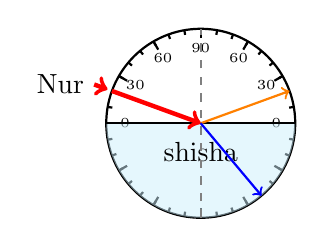
\begin{tikzpicture}[thick, scale=1.2]
    % Optik disk (aylana)
    \draw (0,0) circle (1);
    
    % Gradus belgilari (har 10 gradusda)
    \foreach \a in {0,10,...,350}
        \draw (\a:0.95) -- (\a:1);
    
    % Asosiy sonli belgilar (0, 30, 60, 90)
    \foreach \a in {0, 30, 60, 90, 120, 150, 180, 210, 240, 270, 300, 330}
        \draw (\a:0.9) -- (\a:1);
    
    \node at (0:0.8) {\tiny 0};
    \node at (30:0.8) {\tiny 30};
    \node at (60:0.8) {\tiny 60};
    \node at (90:0.8) {\tiny 90};
    \node at (180:0.8) {\tiny 0};
    \node at (150:0.8) {\tiny 30};
    \node at (120:0.8) {\tiny 60};

    % Shisha plastinka (pastki yarim doira)
    \fill[cyan!20, opacity=0.5] (0,0) -- (1,0) arc (0:-180:1) -- cycle;
    \draw (-1,0) -- (1,0); % Sirt chizig'i
    \node at (0, -0.3) {shisha};

    % Normal (tik chiziq)
    \draw[dashed, gray] (0,-1) -- (0,1);

    % Tushayotgan nur (20 gradus belgisi ustida, normaldan 70 gradusda)
    \draw[red, ultra thick, <-] (0,0) -- (160:1);
    \draw[red, ultra thick, ->] (160:1.2) -- (160:1.05); % Ko'rsatkich strelka
    
    % Qaytgan nur
    \draw[orange, thick, ->] (0,0) -- (20:1);
    
    % Singan nur (taxminan 40 gradus normaldan)
    \draw[blue, thick, ->] (0,0) -- (-50:1);

    % Burchak belgilari
    \node[left] at (160:1.2) {Nur};

\end{tikzpicture}

\begin{enumerate}[label=\Alph*)]
\item $50^\circ$
\item $70^\circ$
\item $40^\circ$
\item $20^\circ$
\item $10^\circ$
\end{enumerate}

\item Qaytgan nur bilan yassi ko‘zgu orasidagi burchak $22^\circ$ bo‘lsa, tushish burchagi qanday?
\begin{enumerate}[label=\Alph*)]
\item $22^\circ$.
\item $38^\circ$.
\item $58^\circ$.
\item $68^\circ$.
\item $82^\circ$.
\end{enumerate}

\item Gorizontal joylashgan yassi ko‘zgu sirti bilan unga tushayotgan nur orasidagi burchak $20^\circ$ bo‘lsa, qaytish burchagi necha gradus bo‘ladi?
\begin{enumerate}[label=\Alph*)]
\item $20^\circ$.
\item $35^\circ$.
\item $40^\circ$.
\item $55^\circ$.
\item $70^\circ$.
\end{enumerate}

\item Ko‘zgu bilan tushayotgan nur orasidagi burchak $35^\circ$ ga teng. Yorug‘likning qaytish burchagini aniqlang.
\begin{enumerate}[label=\Alph*)]
\item $35^\circ$.
\item $70^\circ$.
\item $50^\circ$.
\item $55^\circ$.
\item $25^\circ$.
\end{enumerate}

\item Yassi ko‘zguga tushayotgan nur bilan undan qaytgan nur orasidagi burchak $20^\circ$ bo‘lsa, nurning tushish burchagi qanday?
\begin{enumerate}[label=\Alph*)]
\item $80^\circ$.
\item $40^\circ$.
\item $30^\circ$.
\item $20^\circ$.
\item $10^\circ$.
\end{enumerate}

\item Tushayotgan va qaytgan nurlar orasidagi burchak $50^\circ$ bo‘lsa, nur qanday burchak ostida tushmoqda?
\begin{enumerate}[label=\Alph*)]
\item $20^\circ$.
\item $40^\circ$.
\item $25^\circ$.
\item $50^\circ$.
\item $100^\circ$.
\end{enumerate}

\item Tushuvchi va qaytuvchi yorug‘lik nurlari orasidagi burchak $\alpha$ bo‘lsa, qaytish burchagi?
\begin{enumerate}[label=\Alph*)]
\item $2\alpha$.
\item $90^\circ-\alpha$.
\item $90^\circ-\alpha/2$.
\item $\alpha$.
\item $\alpha/2$.
\end{enumerate}

\item Tushayotgan va qaytgan nurlar orasidagi burchak sinusi $0,5$ bo‘lsa, nur qanday burchak ostida tushmoqda?
\begin{enumerate}[label=\Alph*)]
\item $15^\circ$.
\item $75^\circ$.
\item $30^\circ$ yoki $60^\circ$.
\item $15^\circ$ yoki $75^\circ$.
\item $45^\circ$.
\end{enumerate}

\item Agar ikki muhit chegarasiga tushayotgan nurning tushish burchagi $10^\circ$ ga kamaytirsak, tushayotgan va qaytayotgan nurlar orasidagi burchak qanday o‘zgaradi?
\begin{enumerate}[label=\Alph*)]
\item $5^\circ$ kamayadi.
\item $10^\circ$ kamayadi.
\item o‘zgarmaydi.
\item $20^\circ$ kamayadi.
\item TJY.
\end{enumerate}

\item Agar ko‘zgu $15^\circ$ burchakka burilsa, ko‘zgudan qaytgan nur necha gradusga buriladi?
\begin{enumerate}[label=\Alph*)]
\item 15.
\item 45.
\item 30.
\item 60.
\item 0.
\end{enumerate}

\item Yassi ko‘zgu $\alpha=28^\circ$ burchakka burilsa, ko‘zgudan qaytgan nur qanday burchakka buriladi?
\begin{enumerate}[label=\Alph*)]
\item $84^\circ$.
\item $56^\circ$.
\item $28^\circ$.
\item $14^\circ$.
\item $7^\circ$.
\end{enumerate}

\item Yassi ko‘zgudan qaytayotgan nur ko‘zguning burilishi natijasida dastlabki yo‘nalishdan $\alpha$ burchakka o‘tdi. Ko‘zgu qanday burchakka burilgan?
\begin{enumerate}[label=\Alph*)]
\item $2\alpha$.
\item $\alpha$.
\item 0.
\item $0,25\alpha$.
\item $0,5\alpha$.
\end{enumerate}

\item Yassi ko‘zguga yorug‘lik nuri $22^\circ$ burchak ostida tushmoqda. Agar tushgan nur holati o‘zgartirilmasdan ko‘zgu burilganda, nurning tushish burchagi $36^\circ$ bo‘lib qolsa, qaytgan nur qanday burchakka burilgan?
\begin{enumerate}[label=\Alph*)]
\item $11^\circ$.
\item $14^\circ$.
\item $18^\circ$.
\item $28^\circ$.
\item $6^\circ$.
\end{enumerate}

\item Quyoshning gorizontal balandligi $46^\circ$ ni tashkil etadi. Yassi ko‘zgudan qaytgan quyosh nuri yuqoriga vertikal ravishda yo‘nalishi uchun uning ko‘zguga tushish burchagi qanday bo‘lishi kerak?
\begin{enumerate}[label=\Alph*)]
\item $22^\circ$.
\item $26^\circ$.
\item $28^\circ$.
\item $60^\circ$.
\item $68^\circ$.
\end{enumerate}

\item Quyosh nuri yer sirti bilan $40^\circ$ burchak hosil qiladi. Nurni yer sirtiga tik qo‘yilgan ingichka quvur ichiga yo‘naltirish uchun yassi ko‘zguni gorizontga nisbatan qanday burchak ostida joylashtirish kerak?
\begin{enumerate}[label=\Alph*)]
\item $60^\circ$.
\item $65^\circ$.
\item $70^\circ$.
\item $80^\circ$.
\item $40^\circ$.
\end{enumerate}

\item Ikki yassi ko‘zgu o‘zaro $60^\circ$ burchak hosil qiladi. Birinchi ko‘zgudan qaytgan nur ikkinchi ko‘zgu sirtiga perpendikular tushishi uchun, nurning birinchi ko‘zguga tushish burchagi qanday bo‘lishi kerak?
\begin{enumerate}[label=\Alph*)]
\item $15^\circ$.
\item $30^\circ$.
\item $45^\circ$.
\item $60^\circ$.
\item $90^\circ$.
\end{enumerate}

\item Ko‘zgular orasidagi burchak $\alpha$ necha gradus?

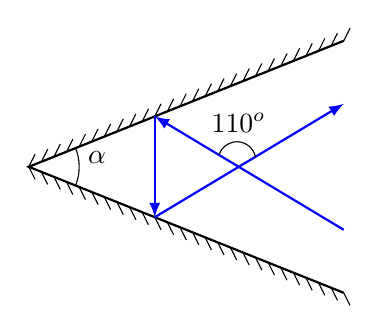
\begin{tikzpicture}[scale=0.8,>=latex]
    % Ko'zgularning burchagi (alfa) va nurning kesishish burchagi (70)
    \coordinate (O) at (0,0);
    \coordinate (A) at (5,2);
    \coordinate (B) at (5,-2);
    
    % Ko'zgularni chizish va shtrixlash
    \draw[thick] (A) -- (O) -- (B);
    \foreach \i in {0,0.2,...,5} {
        \draw (O) ++(\i, {0.4*\i}) -- ++(0.1, 0.2);
        \draw (O) ++(\i, {-0.4*\i}) -- ++(0.1, -0.2);
    }

    \draw[thick,->,blue] (5,-1)--(2,0.8);
    \draw[thick,->,blue] (2,0.8)--(2,-0.8);
    \draw[thick,<-,blue] (5,1)--(2,-0.8);
    
    % Burchaklarni belgilash
    \draw (0.8,0) arc (0:22:0.8) node[midway, right] {$\alpha$};
    \draw (0.8,0) arc (0:-22:0.8);
    
    \coordinate (Inter) at (3.1, 0);
    \draw (3.6, 0.15) arc (10:160:0.3) node[midway, above] {$110^o$};
    
\end{tikzpicture}

\begin{enumerate}[label=\Alph*)]
\item 35.
\item 50.
\item 40.
\item 55.
\item 140.
\end{enumerate}

\item O‘zaro $20^\circ$ burchak ostida joylashtirilgan ikkita ko‘zguga biriga yorug‘lik nuri tushmoqda. Bunda ikkala ko‘zgudan qaytgan nur bilan tushgan nur orasidagi burchak qanday bo‘ladi?
\begin{enumerate}[label=\Alph*)]
\item $80^\circ$.
\item $60^\circ$.
\item $40^\circ$.
\item $30^\circ$.
\item $10^\circ$.
\end{enumerate}

\item Ko‘zgu suvga burchak ostida kiritilgan. Agar $\alpha=20^\circ$ bo‘lsa, $\beta$ va $\gamma$ burchaklarni toping.

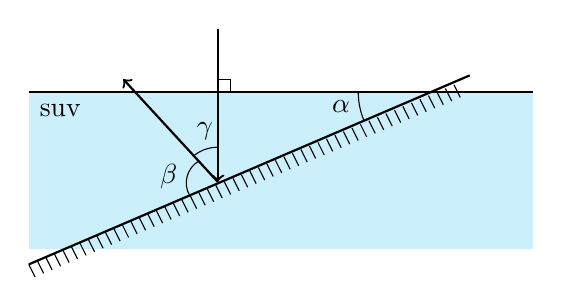
\begin{tikzpicture}[scale=0.8]
    % Suv sathi va ko'zgu
    \fill[cyan!20] (0,0) -- (8,0) -- (8,-2.5) -- (0,-2.5) -- cycle;
    \draw[thick] (0,0) -- (8,0);
    \node at (0.5,-0.3) {suv};
    
    % Qiya ko'zgu
    \coordinate (M1) at (0,-2.74);
    \coordinate (M2) at (7,0.26);
    \draw[thick] (M1) -- (M2);
    
    % Ko'zgu shtrixi
    \foreach \i in {0,0.15,...,7.5} {
        \draw (M1) ++(\i*0.9, \i*0.38) -- ++(0.1, -0.2);
    }
    
    % Nurlar
    \draw[thick, ->] (3,1) -- (3, -1.43);
    \draw[thick, ->] (3, -1.43) -- (1.5, 0.2);
    
    % Burchak belgilari
    \draw (3,0) rectangle (3.2, 0.2); % To'g'ri burchak
    
    \draw (5.23,0) arc (180:202:1.2) node[midway, left] {$\alpha$};
    \draw (2.7, -1.1) arc (120:210:0.4) node[midway, left] {$\beta$};
    \draw (3, -0.88) arc (90:130:0.6) node[midway, above] {$\gamma$};
\end{tikzpicture}

\begin{enumerate}[label=\Alph*)]
\item $\beta=70^\circ$; $\gamma=40^\circ$.
\item $\beta=20^\circ$; $\gamma=60^\circ$.
\item $\beta=50^\circ$; $\gamma=10^\circ$.
\item $\beta=80^\circ$; $\gamma=20^\circ$.
\item $\beta=20^\circ$; $\gamma=50^\circ$.
\end{enumerate}

\item Nurning $L$ ko‘zgudan qaytish burchagini toping.

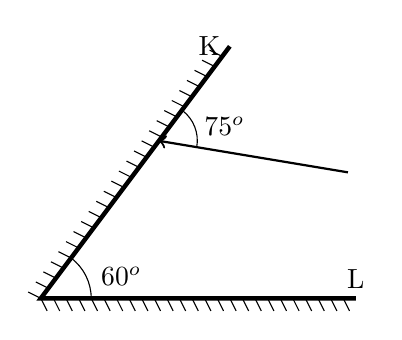
\begin{tikzpicture}[scale=0.8]
    % Koordinatalar
    \coordinate (O) at (0,0);
    \coordinate (L_end) at (5,0);
    \coordinate (K_end) at (3,4);
    
    % Ko'zgularni chizish
    \draw[ultra thick] (K_end) -- (O) -- (L_end);
    \node[left] at (K_end) {K};
    \node[above] at (L_end) {L};
    
    % Shtrixlash (L ko'zgusi)
    \foreach \i in {0,0.2,...,4.8} {
        \draw (\i, 0) -- (\i+0.1, -0.2);
    }
    % Shtrixlash (K ko'zgusi)
    \foreach \i in {0,0.2,...,4.8} {
        \draw (O) ++({0.75*\i/1.25}, \i/1.25) -- ++(-0.2, 0.1);
    }
    
    % Burchaklar
    \draw (0.8,0) arc (0:53:0.8) node[midway, right, xshift=2pt] {$60^o$};
    
    % Kelayotgan nur
    \coordinate (Hit) at (1.875, 2.5);
    \draw[thick, <-] (Hit) -- ++(3, -0.5);
    
    % Nur burchagi
    \draw (Hit) ++(0.6, -0.1) arc (-10:53:0.6) node[midway, right] {$75^o$};
\end{tikzpicture}

\begin{enumerate}[label=\Alph*)]
\item $25^\circ$
\item $35^\circ$
\item $45^\circ$
\item $55^\circ$
\item $65^\circ$
\end{enumerate}

\item Yassi ko‘zguga tushayotgan nur $I$ va qaytgan nur $I'$ bo‘lsa, $\alpha$ burchakni toping.

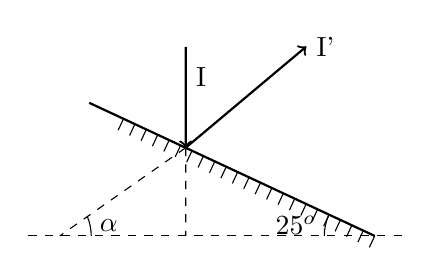
\begin{tikzpicture}[scale=0.8]
    % Gorizontal chiziq
    \draw[dashed] (-0.5,0) -- (5.5,0);
    
    % Ko'zgu (25 gradus)
    \draw[thick] (5,0) -- ++(155:5) coordinate (M);
    \foreach \i in {0,0.2,...,4.5} {
        \draw (5,0) ++(155:\i) -- ++(245:0.2);
    }
    
    % Nurlar
    \coordinate (Hit) at (2, 1.4);
    \draw[thick, ->] (2, 3) -- (Hit) node[pos=0.3, right] {I};
    \draw[thick, ->] (Hit) -- ++(40:2.5) node[right] {I'};
    
    % Burchaklar
    \draw[dashed] (Hit) -- (2,0);
    \draw[dashed] (Hit) -- (0,0);
    \draw (4.2,0) arc (180:155:0.8) node[midway, left] {$25^o$};
    \draw (0.5,0) arc (0:23:0.8) node[midway, right] {$\alpha$};
\end{tikzpicture}


\begin{enumerate}[label=\Alph*)]
\item $30^\circ$
\item $40^\circ$
\item $50^\circ$
\item $75^\circ$
\item $12,5^\circ$
\end{enumerate}

\item Rasmlardagi ma’lumotlardan foydalanib, $\alpha$ burchakni toping.

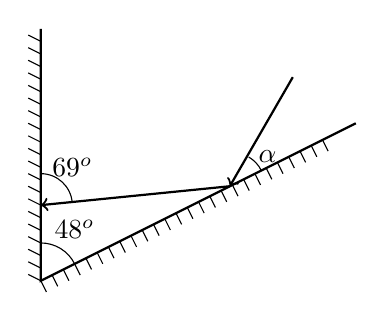
\begin{tikzpicture}[scale=0.8]
    % Ko'zgular
    \coordinate (O) at (0,0);
    \draw[thick] (0,4) -- (O) -- (5,2.5);
    
    % Shtrixlash
    \foreach \i in {0,0.2,...,3.8} \draw (0,\i) -- (-0.2, \i+0.1);
    \foreach \i in {0,0.2,...,5} \draw (O) ++({atan(2.5/5)}:\i) -- ++({atan(2.5/5)-90}:0.2);
    
    % Burchak 48
    \draw (0,0.6) arc (90:{atan(2.5/5)}:0.6) node[midway, above, xshift=5pt] {$48^o$};
    
    % Nur yo'li
    \coordinate (P1) at (3, 1.5);
    \coordinate (P2) at (0, 1.2);
    \draw[thick, <-] (P1) -- ++(60:2);
    \draw[thick, ->] (P1) -- (P2);
    
    % Burchaklar
    \draw (P1) ++(0.5, 0.25) arc (26:60:0.5) node[above, right] {$\alpha$};
    \draw (0, 1.7) arc (90:4:0.5);
    \node at (0.5,1.8) {$69^o$};
\end{tikzpicture}

\begin{enumerate}[label=\Alph*)]
\item $11^\circ$
\item $10,5^\circ$
\item $21^\circ$
\item $42^\circ$
\item $32^\circ$
\end{enumerate}

\item Quyosh nuri yer sirti bilan $36^\circ$ burchak hosil qiladi. Nur yassi ko‘zgudan qaytgach gorizontal yo‘nalishi uchun ko‘zguga tushish burchagi qanday bo‘lishi kerak?

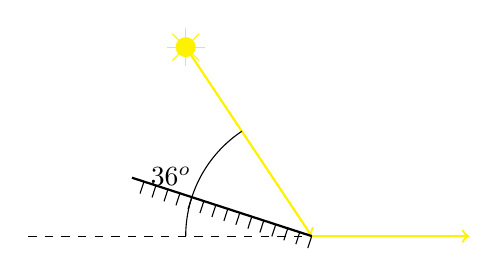
\begin{tikzpicture}[scale=0.8]
    % Gorizontal chiziq
    \draw[dashed] (-2,0) -- (4,0);
    
    % Nur va Quyosh
    \filldraw[yellow] (0.5,3) circle (0.15);
    \foreach \a in {0,45,...,315} \draw[yellow] (0.5,3) -- ++(\a:0.3);
    
    \coordinate (Hit) at (2.5,0);
    \draw[thick, ->,yellow] (0.5,3) -- (Hit);
    \draw[thick, ->, yellow] (Hit) -- (5,0);
    
    % Ko'zgu
    \draw[thick] (Hit) -- ++(162:3);
    
    \foreach \i in {0,0.2,...,2.8} \draw (Hit) ++(162:\i) -- ++(252:0.2);
    
    % Burchak 36
    \draw (0.5,0) arc (180:{180-atan(3/2)}:2) node[midway, left] {$36^o$};
\end{tikzpicture}

\begin{enumerate}[label=\Alph*)]
\item $90^\circ$
\item $84^\circ$
\item $72^\circ$
\item $54^\circ$
\item $36^\circ$
\end{enumerate}

\item Nur yassi ko‘zgudan qaytgach gorizontal yo‘nalishi uchun yer bilan qanday $\alpha$ burchak ostida qo‘yish kerak?

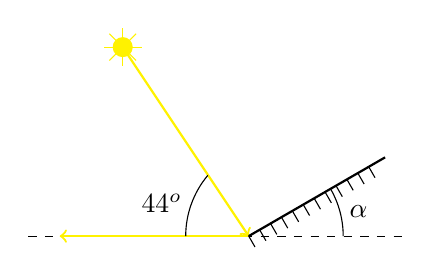
\begin{tikzpicture}[scale=0.8]
    % Gorizontal chiziq
    \draw[dashed] (0,0) -- (6,0);
    
    % Nur va Quyosh
    \filldraw[yellow] (1.5,3) circle (0.15);
    \foreach \a in {0,45,...,315} \draw[yellow] (1.5,3) -- ++(\a:0.3);
    
    \coordinate (Hit) at (3.5,0);
    \draw[thick, ->,yellow] (1.5,3) -- (Hit);
    \draw[thick, ->,yellow] (Hit) -- (0.5,0);
    
    % Ko'zgu
    \draw[thick] (Hit) -- ++(30:2.5);
    \foreach \i in {0,0.2,...,2.3} \draw (Hit) ++(30:\i) -- ++(-60:0.2);
    
    % Burchaklar
    \draw (2.5,0) arc (180:140:1.5) node[midway, left] {$44^o$};
    \draw (5,0) arc (0:30:1.5) node[midway, right] {$\alpha$};
\end{tikzpicture}

\begin{enumerate}[label=\Alph*)]
\item $22^\circ$
\item $56^\circ$
\item $72^\circ$
\item $68^\circ$
\item $11^\circ$
\end{enumerate}

\item O‘zaro $30^\circ$ burchak ostida joylashtirilgan ikkita ko‘zgudan biriga yorug‘lik nuri tushmoqda. Bunda ikkala ko‘zgudan qaytgan nur bilan tushgan nur orasidagi burchak qanday bo‘ladi?
\begin{enumerate}[label=\Alph*)]
\item $90^\circ$.
\item $60^\circ$.
\item $45^\circ$.
\item $30^\circ$.
\item $15^\circ$.
\end{enumerate}

\item Rasmda o‘zaro $\alpha$ burchak ostida joylashgan ko‘zgularga tushib ulardan qaytgan nur yo‘li tasvirlangan. Nur dastlabki yo‘nalishga nisbatan jami qanchaga burilgan?

\begin{tikzpicture}[>=latex, scale=1]
    % Ko'zgularning birlashgan nuqtasi (uchi)
    \coordinate (O) at (0,0);
    % Ko'zgularning oxirgi nuqtalari
    \coordinate (M1_end) at (-3, 2.2);
    \coordinate (M2_end) at (4, 1.8);
    
    % Ko'zgularni chizish
    \draw[thick] (M1_end) -- (O) -- (M2_end);
    
    % Ko'zgularni shtrixlash (orqa tomoni)
    \foreach \t in {0,0.05,...,1} {
        \draw ($(O)!\t!(M1_end)$) -- ++({atan2(2.2,-3)+90}:0.15);
        \draw ($(O)!\t!(M2_end)$) -- ++({atan2(1.8,4)-90}:0.15);
    }
    
    % Nurning ko'zgular bilan to'qnashuv nuqtalari (y=0.9 gorizontal chiziqda)
    % Chap ko'zgu: y = (2.2/-3)*x => x = -0.9 * 3 / 2.2
    \coordinate (P1) at (-1.22, 0.9);
    % O'ng ko'zgu: y = (1.8/4)*x => x = 0.9 * 4 / 1.8
    \coordinate (P2) at (2, 0.9);
    
    % Yorug'lik nurlarini chizish
    \draw[red, thick, <-] (P1) -- (-1.7,2); % Kiruvchi nur
    \draw[red, thick, ->] (P1) -- (P2);        % Gorizontal nur
    \draw[red, thick, ->] (P2) -- ++(50:1.5);  % Chiquvchi nur
    
    % Alfa burchagini belgilash
    \draw (0.45, 0.2) arc (24:143:0.5);
    \node at (0.1, 0.6) {$\alpha$};
    
\end{tikzpicture}

\begin{enumerate}[label=\Alph*)]
\item $90-2\alpha$.
\item $\alpha$.
\item $2\alpha$.
\item $90-\alpha$.
\item $90+\alpha$.
\end{enumerate}

\item Nur dastlabki yo‘nalishiga nisbatan jami qanchaga burilgan?

\begin{tikzpicture}[>=latex, scale=1]
    % Ko'zgularning birlashgan nuqtasi (uchi)
    \coordinate (O) at (0,0);
    % Ko'zgularning oxirgi nuqtalari
    \coordinate (M1_end) at (-3, 2.2);
    \coordinate (M2_end) at (4, 1.8);
    
    % Ko'zgularni chizish
    \draw[thick] (M1_end) -- (O) -- (M2_end);
    
    % Ko'zgularni shtrixlash (orqa tomoni)
    \foreach \t in {0,0.05,...,1} {
        \draw ($(O)!\t!(M1_end)$) -- ++({atan2(2.2,-3)+90}:0.15);
        \draw ($(O)!\t!(M2_end)$) -- ++({atan2(1.8,4)-90}:0.15);
    }
    
    % Nurning ko'zgular bilan to'qnashuv nuqtalari (y=0.9 gorizontal chiziqda)
    % Chap ko'zgu: y = (2.2/-3)*x => x = -0.9 * 3 / 2.2
    \coordinate (P1) at (-1.22, 0.9);
    % O'ng ko'zgu: y = (1.8/4)*x => x = 0.9 * 4 / 1.8
    \coordinate (P2) at (2, 0.9);
    
    % Yorug'lik nurlarini chizish
    \draw[red, thick, <-] (P1) -- (-1.7,2); % Kiruvchi nur
    \draw[red, thick, ->] (P1) -- (P2);        % Gorizontal nur
    \draw[red, thick, ->] (P2) -- ++(50:1.5);  % Chiquvchi nur
    
    % Alfa burchagini belgilash
    \draw (0.45, 0.2) arc (24:143:0.5);
    \node at (0.1, 0.6) {$150^\circ$};
    
\end{tikzpicture}

\begin{enumerate}[label=\Alph*)]
\item $30^\circ$.
\item $300^\circ$.
\item $60^\circ$.
\item $90^\circ$.
\item $75^\circ$.
\end{enumerate}

\item Agar yassi ko‘zguda buyum tasviri ko‘zgudan $70$ cm masofada hosil bo‘lsa, buyum bilan uning tasviri orasidagi masofa necha cm bo‘ladi?
\begin{enumerate}[label=\Alph*)]
\item 35.
\item 70.
\item 140.
\item 105.
\item 2.
\end{enumerate}

\item Yassi ko‘zgu oldida odam turibdi. Agar u ko‘zguga $1$ m yaqinlashsa, odam va uning tasviri orasidagi masofa qanday o‘zgaradi?
\begin{enumerate}[label=\Alph*)]
\item o‘zgarmaydi.
\item 1 m kamayadi.
\item 0,5 m kamayadi.
\item 2 m kamayadi.
\item TJY.
\end{enumerate}

\item Agar bola vertikal joylashgan ko‘zgu tekisligiga $4$ m yaqinlashsa, uning ko‘zgudagi tasviri unga necha metr yaqinlashadi?
\begin{enumerate}[label=\Alph*)]
\item 2.
\item 4.
\item 8.
\item 1.
\item TJY.
\end{enumerate}

\item Agar odamning eng yaxshi ko‘rish masofasi $30$ cm bo‘lsa, o‘zining ko‘zgudagi tasvirini yaxshiroq ko‘rish uchun u ko‘zgudan necha cm masofada turishi kerak?
\begin{enumerate}[label=\Alph*)]
\item 15.
\item 25.
\item 30.
\item 60.
\item TJY.
\end{enumerate}

\item Odam vertikal joylashgan yassi ko‘zgu tekisligiga $2,6$ m yaqinlashsa, u bilan uning tasviri orasidagi masofa qanday o‘zgaradi?
\begin{enumerate}[label=\Alph*)]
\item o‘zgarmaydi.
\item 1,3 m kamayadi.
\item 5,2 m kamayadi.
\item 2,6 m kamayadi.
\item TJY.
\end{enumerate}

\item Odam vertikal joylashgan yassi ko‘zgu tekisligidan $3$ m uzoqlashsa, u bilan uning tasviri orasidagi masofa qanday o‘zgaradi?
\begin{enumerate}[label=\Alph*)]
\item 3 m kattalashadi.
\item 1,5 m kattalashadi.
\item o‘zgarmaydi.
\item 6 m kattalashadi.
\item TJY.
\end{enumerate}

\item Bola yassi ko‘zguda o‘z aksini ko‘rmoqda. Agar u ko‘zguga $0,6$ m/s tezlik bilan yaqinlashsa, uning aksi unga necha m/s tezlik bilan yaqinlashadi?
\begin{enumerate}[label=\Alph*)]
\item 1,2.
\item 1,1.
\item 1.
\item 0,9.
\item 0,6.
\end{enumerate}

\item Kishi yassi ko‘zguga $1$ m/s tezlik bilan yaqinlashsa, u o‘z tasviri unga qanday tezlik (m/s) bilan yaqinlashadi?
\begin{enumerate}[label=\Alph*)]
\item 1,5.
\item 2,5.
\item 3.
\item 2.
\item 2.
\end{enumerate}

\item Yassi ko‘zgu o‘z tekisligiga tik ravishda $1,5$ cm/s tezlik bilan yorug‘lik manbai tomon harakatlanmoqda. Ko‘zgudagi tasviri o‘zgarmas bo‘lishi uchun yorug‘lik manbai necha cm/s tezlik bilan va qaysi tomonga harakatlanishi kerak?
\begin{enumerate}[label=\Alph*)]
\item 1,5, ko‘zgudan.
\item 3, ko‘zguga.
\item 3, ko‘zgudan.
\item 1,5, ko‘zguga.
\item 0,75, ko‘zgudan.
\end{enumerate}

\item Qizcha ko‘zguga tik yo‘nalishda $0,5$ m/s tezlik bilan yaqinlashmoqda. Qizchaning tasviri unga va ko‘zguga qanday tezliklar (m/s) bilan yaqinlashadi?
\begin{enumerate}[label=\Alph*)]
\item 1; 0,5.
\item 0,5; 0,5.
\item 1; 1.
\item 0,5; 1.
\item TJY.
\end{enumerate}

\item Bola tasvirining yerga nisbatan tezligini toping.
\begin{enumerate}[label=\Alph*)]
\item $2v$.
\item $3v$.
\item $4v$.
\item $v$.
\item $v/2$.
\end{enumerate}

\item OA ko‘zgu chizma tekisligiga tik bo‘lgan va O nuqtadan o‘tuvchi o‘q atrofida $\omega$ burchak tezlik bilan aylanadi. $OS=l$ bo‘lsa S nuqtaning tasviri rasmda ko‘rsatilgan paytda qanday tezlik bilan harakatlanadi?

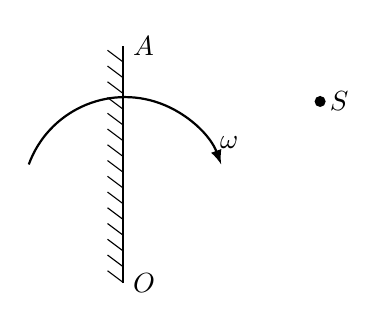
\begin{tikzpicture}[>=latex]
    % Vertikal ko'zgu AO
    \coordinate (O) at (0,0);
    \coordinate (A) at (0,3);
    \draw[thick] (O) -- (A);
    \node[right] at (A) {$A$};
    \node[right] at (O) {$O$};
    
    % Ko'zguning orqa tomonini shtrixlash
    \foreach \y in {0,0.2,...,2.8} {
        \draw (0,\y) -- (-0.2, \y+0.15);
    }
    
    % S nuqta
    \fill (2.5, 2.3) circle (2pt) node[right] {$S$};
    
    % Aylanish strelkasi (omega)
    \draw[thick, ->] (-1.2, 1.5) arc (160:20:1.3) node[pos=0.9,  right] {$\omega$};
\end{tikzpicture}

\begin{enumerate}[label=\Alph*)]
\item $2\omega l$.
\item $\omega l$.
\item $\omega l/2$.
\item $3\omega l/2$.
\item $l/\omega$.
\end{enumerate}

\item A nuqta gorizontal yo‘nalishda $v_1=3$ m/s, MN yassi ko‘zgu vertikal yo‘nalishda $v_2=4$ m/s tezlik bilan rasmda ko‘rsatilgandek harakatlanmoqda. A nuqtaning ko‘zgudagi tasvirining tezligini (m/s) toping.

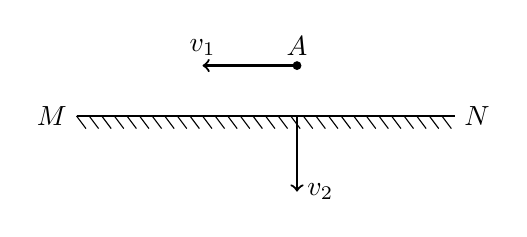
\begin{tikzpicture}[scale=0.8]
    % Gorizontal ko'zgu MN
    \coordinate (M) at (0,0);
    \coordinate (N) at (6,0);
    \draw[thick] (M) -- (N);
    \node[left] at (M) {$M$};
    \node[right] at (N) {$N$};
    
    % Shtrixlash
    \foreach \x in {0,0.2,...,5.8} {
        \draw (\x, 0) -- (\x+0.15, -0.2);
    }
    
    % A nuqta va v1 tezlik
    \fill (3.5, 0.8) circle (2pt) node[above] {$A$};
    \draw[thick, ->] (3.5, 0.8) -- (2, 0.8) node[above] {$v_1$};
    
    % v2 vektori (pastga yo'nalgan)
    \draw[thick, ->] (3.5, 0) -- (3.5, -1.2) node[right] {$v_2$};
\end{tikzpicture}

\begin{enumerate}[label=\Alph*)]
\item 5.
\item $\sqrt{52}$.
\item 8.
\item $\sqrt{73}$.
\item 10.
\end{enumerate}

\item A nuqta gorizontal yo‘nalishda $v_1=8$ m/s, MN yassi ko‘zgu vertikal yo‘nalishda $v_2=3$ m/s tezlik bilan rasmda ko‘rsatilgandek harakatlanmoqda. A nuqtaning ko‘zgudagi tasvirining tezligini (m/s) toping.

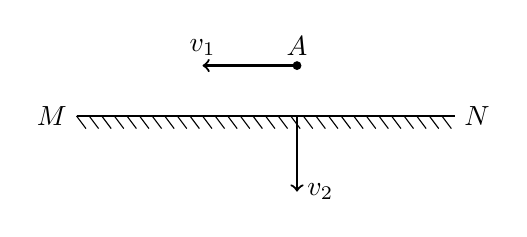
\begin{tikzpicture}[scale=0.8]
    % Gorizontal ko'zgu MN
    \coordinate (M) at (0,0);
    \coordinate (N) at (6,0);
    \draw[thick] (M) -- (N);
    \node[left] at (M) {$M$};
    \node[right] at (N) {$N$};
    
    % Shtrixlash
    \foreach \x in {0,0.2,...,5.8} {
        \draw (\x, 0) -- (\x+0.15, -0.2);
    }
    
    % A nuqta va v1 tezlik
    \fill (3.5, 0.8) circle (2pt) node[above] {$A$};
    \draw[thick, ->] (3.5, 0.8) -- (2, 0.8) node[above] {$v_1$};
    
    % v2 vektori (pastga yo'nalgan)
    \draw[thick, ->] (3.5, 0) -- (3.5, -1.2) node[right] {$v_2$};
\end{tikzpicture}

\begin{enumerate}[label=\Alph*)]
\item 10.
\item $\sqrt{52}$.
\item 8.
\item $\sqrt{73}$.
\item 20.
\end{enumerate}

\item Bo‘yi $1,6$ m bo‘lgan qiz boshini holatini o‘zgartirmasdan o‘zining vertikal yassi ko‘zgudagi aksini to‘liqincha ko‘rish uchun ko‘zguning balandligi kamida necha metr bo‘lishi kerak?
\begin{enumerate}[label=\Alph*)]
\item 1,6.
\item 0,8.
\item 0,4.
\item 2,4.
\item javob qiz va ko‘zgu orasidagi masofaga bog‘liq.
\end{enumerate}

\item Yassi ko‘zgu oldida turgan, bo‘yi $l$ bo‘lgan kishi o‘zining to‘liq tasvirini ko‘rishi uchun ko‘zguning o‘lchami (balandligi) kamida qancha bo‘lishi kerak?
\begin{enumerate}[label=\Alph*)]
\item $l/2$.
\item $2l/3$.
\item $l/4$.
\item $l$.
\item $l/3$.
\end{enumerate}

\item G nuqtadan ko‘zguga qarab devorning necha metr balandligini ko‘rish mumkin?

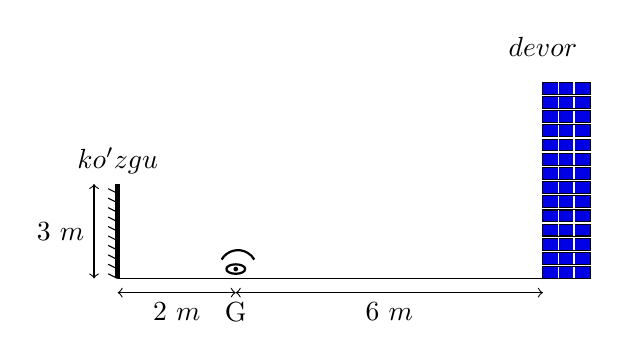
\begin{tikzpicture}[scale=0.6]
    % Yer chizig'i
    \draw (0,0) -- (10,0);
    
    % Ko'zgu (3m balandlikda)
    \draw[ultra thick] (0,0) -- (0,2);
    \foreach \y in {0,0.2,...,1.8} \draw (0,\y) -- (-0.2, \y+0.1);
    \draw[<->] (-0.5, 0) -- (-0.5, 2) node[midway, left] {$3 \ m$};
    \node[above] at (0,2) {$ko'zgu$};
    
    % Kuzatuvchi ko'zi (G)
    \coordinate (G) at (2.5, 0);
    \draw[thick] (G) ++(-0.3,0.4) arc (150:30:0.4); % Qosh
    \draw[thick] (G) ++(-0.2,0.2) arc (180:360:0.2 and 0.1); % Ko'z osti
    \draw[thick] (G) ++(-0.2,0.2) arc (180:0:0.2 and 0.1); % Ko'z usti
    \fill (G) ++(0,0.2) circle (0.05); % Qorachiq
    \node[below=5pt] at (G) {G};
    
    % Masofalar
    \draw[<->] (0,-0.3) -- (2.5,-0.3) node[midway, below] {$2 \ m$};
    \draw[<->] (2.5,-0.3) -- (9,-0.3) node[midway, below] {$6 \ m$};
    
    % Devor (G'ishtli)
    \node[above] at (9, 4.5) {$devor$};
    \foreach \y in {0,0.3,...,4.2} {
        \draw[fill=blue!90!black] (9,\y) rectangle (10,\y+0.25);
        \draw[white, thin] (9.33,\y) -- (9.33, \y+0.25);
        \draw[white, thin] (9.66,\y) -- (9.66, \y+0.25);
    }
\end{tikzpicture}

\begin{enumerate}[label=\Alph*)]
\item 10.
\item 15.
\item 20.
\item 8.
\item 5.
\end{enumerate}

\setcounter{enumi}{48}

\item Ikki yassi shisha plastina bir-biridan $a$ masofada parallel qo‘yilgan. Rasmdan foydalanib, $A$ jismning plastinalardagi tasvirlari orasidagi masofani toping. $A$ jismdan birinchi plastinagacha bo‘lgan masofa $b$ ga teng.

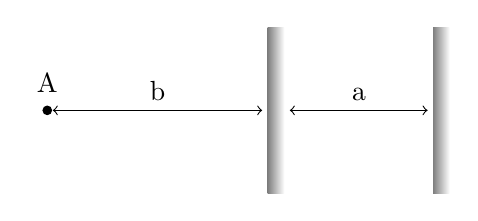
\begin{tikzpicture}[scale=0.7]
    % A nuqta
    \fill (0,0) circle (2.5pt) node[above=3pt] {A};
    
    % Ko'zgular (Parallel)
    \fill[left color=gray, right color=white] (4,-1.5) rectangle (4.3, 1.5);
    \fill[left color=gray, right color=white] (7,-1.5) rectangle (7.3, 1.5);
    
    % Masofalar va strelkalar
    \draw[<->] (0.1,0) -- (3.9,0) node[midway, above] {b};
    \draw[<->] (4.4,0) -- (6.9,0) node[midway, above] {a};
\end{tikzpicture}

\begin{enumerate}[label=\Alph*)]
\item $a+b$.
\item $2b$.
\item $2a$.
\item $b-a$.
\item $4b$.
\end{enumerate}

\item $N_1O$ va $N_2O$ yassi ko‘zgular bir-biriga nisbatan $120^\circ$ burchak ostida joylashgan. Yorug‘lik manbai ko‘zgular kesishgan chiziqdan $12$ cm masofada, ko‘zguga nisbatan simmetrik joylashgan. Yorug‘lik manbaining ko‘zgulardagi hosil bo‘lgan mavhum tasvirlari orasidagi masofa qanday (cm)?

\begin{tikzpicture}[scale=0.6]
    % Markaz
    \coordinate (O) at (0,2.5);
    \node[above] at (O) {O};
    
    % Ko'zgular
    \draw[thick] (O) -- (-3,-1) node[below left] {$N_1$};
    \draw[thick] (O) -- (3,-1) node[below right] {$N_2$};
    
    % Shtrixlash
    \foreach \t in {0.1, 0.2, ..., 1} {
        \draw ($(O)!\t!(-3,-1)$) -- ++(120:0.2);
        \draw ($(O)!\t!(3,-1)$) -- ++(60:0.2);
    }
    
    % S nuqta va nurlar
    \fill (0,0) circle (2pt) node[below] {S};
    \draw[dashed, thick] (0,0) -- (0,2.5); % Vertikal normal
    \draw[dashed, thick] (0,0) -- (2.5, 1.9); % Akslanish nuri
\end{tikzpicture}

\begin{enumerate}[label=\Alph*)]
\item 12.
\item 17.
\item 20,8.
\item 24.
\item TJY.
\end{enumerate}

\item Ikki yassi ko‘zgular bir-biriga nisbatan $120^\circ$ burchak ostida joylashgan. Yorug‘lik manbai har ikki ko‘zgudan $20$ cm uzoqlikda ular orasida joylashgan. Yorug‘lik manbaining ko‘zgularda hosil bo‘lgan tasvirlari orasidagi masofani qanday (cm)?
\begin{enumerate}[label=\Alph*)]
\item 40.
\item 34,6.
\item 50.
\item 69,2.
\item 10.
\end{enumerate}

\item Ikki yassi ko‘zgular bir-biriga nisbatan $90^\circ$ burchak ostida joylashgan. Yorug‘lik manbai biridan $5$ cm, ikkinchisidan $12$ cm masofada joylashgan. Yorug‘lik manbaining ko‘zgularda hosil bo‘lgan tasvirlari orasidagi masofani qanday (cm)?
\begin{enumerate}[label=\Alph*)]
\item 13.
\item 20.
\item 26.
\item 24.
\item 6.
\end{enumerate}

\item $L$ nuqtadan taralgan nur ko‘zgulardan qaytgach qaysi nuqtaga tushadi?

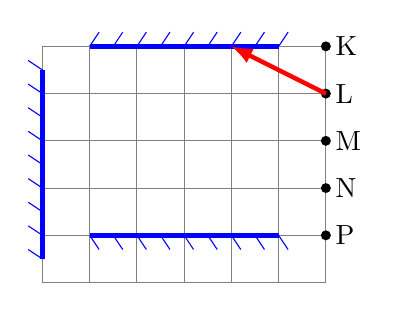
\begin{tikzpicture}[scale=0.6]
    % Kataklar (Grid)
    \draw[step=1, gray, thin] (0,0) grid (6,5);
    
    % Ko'zgular (Chap, Yuqori, Pastki)
    \draw[ultra thick,blue] (0,0.5) -- (0,4.5); % Chap
    \draw[ultra thick,blue] (1,5) -- (5,5);     % Yuqori
    \draw[ultra thick, blue] (1,1) -- (5,1);     % Pastki
    
    % Ko'zgu shtrixlari
    \foreach \y in {0.5, 1, ..., 4.5} \draw[blue] (0, \y) -- (-0.3, \y+0.2);
    \foreach \x in {1, 1.5, ..., 5} {
        \draw[blue] (\x, 5) -- (\x+0.2, 5.3);
        \draw[blue] (\x, 1) -- (\x+0.2, 0.7);
    }
    
    % Nuqtalar (O'ng tomonda)
    \fill (6,5) circle (3pt) node[right] {K};
    \fill (6,4) circle (3pt) node[right] {L};
    \fill (6,3) circle (3pt) node[right] {M};
    \fill (6,2) circle (3pt) node[right] {N};
    \fill (6,1) circle (3pt) node[right] {P};
    
    % Nur (L dan tushayotgan)
    \draw[ultra thick, ->, red, >=latex] (6,4) -- (4,5);
\end{tikzpicture}

\begin{enumerate}[label=\Alph*)]
\item L.
\item M.
\item N.
\item P.
\item K.
\end{enumerate}

\item Buyum o‘zaro tik joylashgan ikkita yassi ko‘zgular orasida joylashgan (rasmga q.). Ko‘zgularda buyumning nechta tasviri ko‘rinadi?

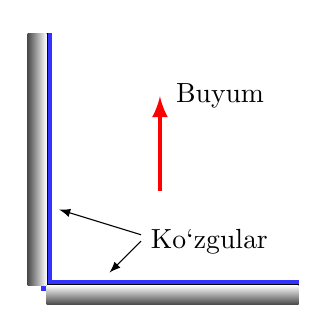
\begin{tikzpicture}[scale=0.8,>=latex]
    % Ko'zgularni chizish (L-shakl)
    % Rasmdagi gradient effektini berish uchun qalin chiziqlar ishlatamiz
    \draw[line width=4pt, blue!80] (0,4) -- (0,0) -- (4,0);
    \draw[thick] (0,4) -- (0,0) -- (4,0);
    
    % Buyum (Arrow)
    \draw[ultra thick,red, ->] (1.8, 1.5) -- (1.8, 3);
    \node[right] at (1.9, 3) {Buyum};
    
    % "Ko'zgular" yozuvi va ko'rsatkich chiziqlari
    \node[right] at (1.5, 0.7) {Ko`zgular};
    \draw[thin,->] (1.5, 0.7) -- (1, 0.2);
    \draw[thin,->] (1.5, 0.8) -- (0.2, 1.2);
    
    % Ko'zgularning orqa tomonini quyuqlashtirish (gradient simulyatsiyasi)
    \fill[left color=black!70, right color=white] (-0.3, 0) rectangle (0, 4);
    \fill[top color=white, bottom color=black!70] (0, -0.3) rectangle (4, 0);
\end{tikzpicture}

\begin{enumerate}[label=\Alph*)]
\item Cheksiz ko‘p.
\item 2.
\item 3.
\item 4.

\end{enumerate}

\end{enumerate}

\begin{center}
\renewcommand{\arraystretch}{1.2}
\begin{tabular}{|c|c|c|c|c|c|c|c|c|c|}
\hline
1d & 2e & 3e & 4e & 5b & 6d & 7e & 8d & 9e & 10c \\
\hline
11e & 12d & 13d & 14c & 15b & 16e & 17d & 18a & 19b & 20d \\
\hline
21d & 22c & 23a & 24a & 25b & 26c & 27c & 28d & 29b & 30c \\
\hline
31c & 32c & 33d & 34c & 35a & 36c & 37d & 38a & 39e & 40c \\
\hline
41a & 42b & 43a & 44d & 45a & 46b & 47a & 48b & 49c & 50c \\
\hline
51a & 52b & 53c & 54c & & & & & & \\
\hline
\end{tabular}
\end{center}





\section{Yorug‘likning sinishi}

\begin{enumerate}
\item Chizmalarning qaysi birida tushish burchagi $\alpha$, qaytish burchagi $\beta$ va sinish burchagi $\gamma$ to‘g‘ri ko‘rsatilgan?

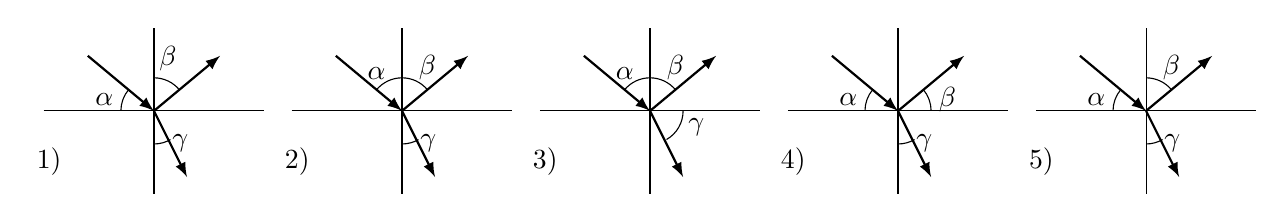
\begin{tikzpicture}[>=latex, scale=0.7]
    % --- 1-rasm ---
    \begin{scope}[shift={(0,0)}]
        \draw (-2,0) -- (2,0); \draw (0,-1.5) -- (0,1.5);
        \draw[thick, ->] (-1.2,1) -- (0,0); \draw[thick, ->] (0,0) -- (1.2,1); \draw[thick, ->] (0,0) -- (0.6,-1.2);
        \draw (-0.6,0) arc (180:140:0.6) node[midway, left] {$\alpha$};
        \draw (0,0.6) arc (90:40:0.6) node[midway, above] {$\beta$};
        \draw (0,-0.6) arc (270:300:0.6) node[midway, right] {$\gamma$};
        \node[below left] at (-1.5,-0.5) {1)};
    \end{scope}

    % --- 2-rasm ---
    \begin{scope}[shift={(4.5,0)}]
        \draw (-2,0) -- (2,0); 
        \draw (0,-1.5) -- (0,1.5);
        \draw[thick, ->] (-1.2,1) -- (0,0); 
        \draw[thick, ->] (0,0) -- (1.2,1); 
        \draw[thick, ->] (0,0) -- (0.6,-1.2);
        \draw (0,0.6) arc (90:140:0.6) node[above] {$\alpha$};
        \draw (0,0.6) arc (90:40:0.6) node[above] {$\beta$};
        \draw (0,-0.6) arc (270:300:0.6) node[midway, right] {$\gamma$};
        \node[below left] at (-1.5,-0.5) {2)};
    \end{scope}

    % --- 3-rasm ---
    \begin{scope}[shift={(9,0)}]
        \draw (-2,0) -- (2,0); 
        \draw (0,-1.5) -- (0,1.5);
        \draw[thick, ->] (-1.2,1) -- (0,0); 
        \draw[thick, ->] (0,0) -- (1.2,1); 
        \draw[thick, ->] (0,0) -- (0.6,-1.2);
        \draw (0,0.6) arc (90:140:0.6) node[above] {$\alpha$};
        \draw (0,0.6) arc (90:40:0.6) node[above] {$\beta$};
        \draw (0.6,0) arc (0:-60:0.6) node[midway, right] {$\gamma$};
        \node[below left] at (-1.5,-0.5) {3)};
    \end{scope}

    % --- 4-rasm ---
    \begin{scope}[shift={(13.5,0)}]
        \draw (-2,0) -- (2,0); \draw (0,-1.5) -- (0,1.5);
        \draw[thick, ->] (-1.2,1) -- (0,0); \draw[thick, ->] (0,0) -- (1.2,1); \draw[thick, ->] (0,0) -- (0.6,-1.2);
        \draw (-0.6,0) arc (180:140:0.6) node[midway, left] {$\alpha$};
        \draw (0.6,0) arc (0:40:0.6) node[midway, right] {$\beta$};
        \draw (0,-0.6) arc (270:300:0.6) node[midway, right] {$\gamma$};
        \node[below left] at (-1.5,-0.5) {4)};
    \end{scope}

    % --- 5-rasm ---
    \begin{scope}[shift={(18,0)}]
        \draw (-2,0) -- (2,0); 
        \draw (0,-1.5) -- (0,1.5);
        \draw[thick, ->] (-1.2,1) -- (0,0); 
        \draw[thick, ->] (0,0) -- (1.2,1); 
        \draw[thick, ->] (0,0) -- (0.6,-1.2);
        \draw (-0.6,0) arc (180:140:0.6) node[midway, left] {$\alpha$};
        \draw (0,0.6) arc (90:40:0.6) node[above] {$\beta$};
        \draw (0,-0.6) arc (270:300:0.6) node[midway, right] {$\gamma$};
        \node[below left] at (-1.5,-0.5) {5)};
    \end{scope}
\end{tikzpicture}

\begin{enumerate}[label=\Alph*)]
\item 1.
\item 2.
\item 3.
\item 4.
\item 5.
\end{enumerate}

\item Yorug‘lik nuri havodan absolyut sindirish ko‘rsatkichi $\sqrt{3}$ bo‘lgan muhitga o‘tdi. Bunda tushish burchagi $60^\circ$ ga teng bo‘lsa, sinish burchagini toping.
\begin{enumerate}[label=\Alph*)]
\item $50^\circ$
\item $60^\circ$
\item $70^\circ$
\item $30^\circ$
\item $90^\circ$
\end{enumerate}

\item Yorug‘lik nuri absolyut sindirish ko‘rsatkichi $\sqrt{3}$ bo‘lgan birinchi muhitdan, absolyut sindirish ko‘rsatkichi $\sqrt{2}$ ga teng bo‘lgan muhitga sinib o‘tdi. Agar sinish burchagi $60^\circ$ ga teng bo‘lsa, tushish burchagini toping.
\begin{enumerate}[label=\Alph*)]
\item $50^\circ$
\item $60^\circ$
\item $45^\circ$
\item $30^\circ$
\item $90^\circ$
\end{enumerate}

\item Yorug‘lik nuri absolyut sindirish ko‘rsatkichi $\sqrt{2}$ ga teng bo‘lgan birinchi muhitdan ikkinchi muhitga sinib o‘tdi. Bunda tushish burchagi $30^\circ$ ga, sinish burchagi esa $45^\circ$ ga teng. Ikkinchi muhitning absolyut sindirish ko‘rsatkichini toping.
\begin{enumerate}[label=\Alph*)]
\item $\sqrt{2}$
\item $\sqrt{3}$
\item $1$
\item $2$
\item $3$
\end{enumerate}

\item Yorug‘lik nuri absolyut sindirish ko‘rsatkichi $2$ bo‘lgan birinchi muhitdan, absolyut sindirish ko‘rsatkichi $2\sqrt{2}$ ga teng bo‘lgan muhitga sinib o‘tdi. Agar sinish burchagi $30^\circ$ ga teng bo‘lsa, tushish burchagini toping.
\begin{enumerate}[label=\Alph*)]
\item $50^\circ$
\item $60^\circ$
\item $45^\circ$
\item $30^\circ$
\item $90^\circ$
\end{enumerate}

\item Yorug‘lik nuri absolyut sindirish ko‘rsatkichi $3$ ga teng bo‘lgan birinchi muhitdan ikkinchi muhitga sinib o‘tdi. Bunda tushish burchagi $30^\circ$ ga, sinish burchagi esa $60^\circ$ ga teng. Ikkinchi muhitning absolyut sindirish ko‘rsatkichini toping.
\begin{enumerate}[label=\Alph*)]
\item $\sqrt{2}$
\item $\sqrt{3}$
\item $1$
\item $2$
\item $3$
\end{enumerate}

\item Yorug‘lik nuri birinchi muhitdan absolyut sindirish ko‘rsatkichi $2\sqrt{2}$ ga teng bo‘lgan ikkinchi muhitga sinib o‘tdi. Bunda tushish burchagi $45^\circ$ ga, sinish burchagi esa $30^\circ$ ga teng. Birinchi muhitning absolyut sindirish ko‘rsatkichini toping.
\begin{enumerate}[label=\Alph*)]
\item $\sqrt{2}$
\item $\sqrt{3}$
\item $1$
\item $2$
\item $3$
\end{enumerate}

\item Yorug‘lik nurining 1-muhitdan 2-muhitga o‘tishida tushish burchagi $30^\circ$, sinish burchagi esa $60^\circ$. 2-muhitning 1-muhitga nisbatan sindirish ko‘rsatkichi qanday?
\begin{enumerate}[label=\Alph*)]
\item $0,5$
\item $2$
\item $\sqrt{3}$
\item $\sqrt{3}/3$
\item TJY.
\end{enumerate}

\item Nur shishadan havoga o‘tmoqda. Tushish burchagi $30^\circ$. Nur singanda, o‘z yo‘nalishini $30^\circ$ ga o‘zgartirgan bo‘lsa, shishaning sindirish ko‘rsatkichi qanday?
\begin{enumerate}[label=\Alph*)]
\item $\sqrt{2}$
\item $\sqrt{3}$
\item $2$
\item $\sqrt{2}/2$
\item $1,5$
\end{enumerate}

\item Yorug‘lik nuri havodan absolyut sindirish ko‘rsatkichi $\sqrt{2}$ bo‘lgan muhitga o‘tdi. Bunda tushish burchagi $45^\circ$ ga teng bo‘lsa, sinish burchagini toping.
\begin{enumerate}[label=\Alph*)]
\item $90^\circ$
\item $60^\circ$
\item $45^\circ$
\item $30^\circ$
\item $0^\circ$
\end{enumerate}

\item Yorug‘lik nuri havodan turli muhitlarning yassi sirtiga tushganda, qaytgan va singan nurlar orasidagi burchak tushish burchagidan $1,5$ marta katta bo‘ldi. Agar tushish burchagi $60^\circ$ bo‘lsa, sinish burchagi qanday bo‘ladi?
\begin{enumerate}[label=\Alph*)]
\item $90^\circ$
\item $60^\circ$
\item $45^\circ$
\item $30^\circ$
\item $0^\circ$
\end{enumerate}

\item Rasmdagi ma’lumotlardan $n_2$ ni toping. $\sin53^\circ=0,8$.

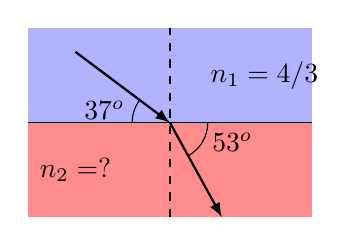
\begin{tikzpicture}[scale=0.6,>=latex]
    % Muhitlar
    \fill[blue!30] (-3,0) rectangle (3,2);   % n1 muhit
    \fill[red!45] (-3,0) rectangle (3,-2);  % n2 muhit
    \draw (-3,0) -- (3,0);
    \draw[dashed] (0,-2) -- (0,2);
    
    % Nurlar
    \draw[thick, ->] (-2, 1.5) -- (0,0);
    \draw[thick, ->] (0,0) -- (1.1, -2);
    
    % Burchaklar (53 gradus sirtga nisbatan)
    \draw (-0.8,0) arc (180:143:0.8) node[midway, left] {$37^o$};
    \draw (0.8,0) arc (0:-61:0.8) node[midway, right] {$53^o$};
    
    % Yozuvlar
    \node at (2,1) {$n_1=4/3$};
    \node at (-2,-1) {$n_2=?$};
\end{tikzpicture}

\begin{enumerate}[label=\Alph*)]
\item $5/3$
\item $25/9$
\item $1$
\item $16/9$
\item $25/16$
\end{enumerate}

\item Nur havodan shisha sirtiga $45^\circ$ burchak ostida tushsa, sinish burchagi necha gradus bo‘ladi? Shisha uchun $n=1,41$.
\begin{enumerate}[label=\Alph*)]
\item $25^\circ$
\item $21^\circ$
\item $30^\circ$
\item $37^\circ$
\item $42^\circ$
\end{enumerate}

\item Havodan shishaga $60^\circ$ burchak ostida yorug‘lik tushmoqda. Agar qaytgan va singan nur orasidagi burchak tushish burchagidan $1,5$ marta katta bo‘lsa, shishaning sindirish ko‘rsatkichi qanday?
\begin{enumerate}[label=\Alph*)]
\item $\sqrt{2}$
\item $\sqrt{3}$
\item $1$
\item $2$
\item $3$
\end{enumerate}

\item Havodan shishaga tushuvchi va qaytgan nurlar orasidagi burchak $60^\circ$. Sinish burchagining sinusini toping? $n=1,5$.
\begin{enumerate}[label=\Alph*)]
\item $2/3$
\item $3/5$
\item $1/2$
\item $1/3$
\item $1/4$
\end{enumerate}

\item Sinish burchagi tushish burchagidan 2 marta kichik bo‘lishi uchun havodan shisha sirtiga yorug‘lik qanday burchak ostida tushishi kerak? $n_{\text{sh}}=\sqrt{3}$.
\begin{enumerate}[label=\Alph*)]
\item $50^\circ$
\item $60^\circ$
\item $70^\circ$
\item $80^\circ$
\item $90^\circ$
\end{enumerate}

\item Yorug‘lik nuri bir muhitdan optik zichligi kattaroq bo‘lgan ikkinchi muhitga sinib o‘tganda ...
\begin{enumerate}[label=\Alph*)]
\item sinish burchagi tushish burchagidan kichikroq bo‘ladi.
\item sinish burchagi tushish burchagidan kattaroq bo‘ladi.
\item sinish burchagi tushish burchagiga teng bo‘ladi.
\item javob tushish burchagiga bog‘liq.
\item TJY.
\end{enumerate}

\item Qaysi chizmada yorug‘lik nurining optik zichligi kattaroq bo‘lgan muhitdan optik zichligi kichikroq bo‘lgan muhitga o‘tishi tasvirlangan?

\begin{tikzpicture}[>=latex, scale=0.8]
    % --- 1-rasm (Buralish uzoqlashgan) ---
    \begin{scope}[shift={(0,0)}]
        \draw (-2,0) -- (2,0);
        \draw[dashed] (0,-1.5) -- (0,1.5);
        \draw[thick, ->] (-1, 1.2) -- (0,0); % Tushayotgan
        \draw[thick, ->] (0,0) -- (1.4, -1);  % Sinayotgan (normallashgan uzoqlashgan)
        \node at (-1,-1) {1};
    \end{scope}

    % --- 2-rasm (Normalga yaqinlashgan) ---
    \begin{scope}[shift={(5,0)}]
        \draw (-2,0) -- (2,0);
        \draw[dashed] (0,-1.5) -- (0,1.5);
        \draw[thick, ->] (-1.5, 0.7) -- (0,0);
        \draw[thick, ->] (0,0) -- (0.5, -1.3); % Normalga yaqinlashgan
        \node at (-1,-1) {2};
    \end{scope}

    % --- 3-rasm (Dikroq tushib, uzoqlashgan) ---
    \begin{scope}[shift={(10,0)}]
        \draw (-2,0) -- (2,0);
        \draw[dashed] (0,-1.5) -- (0,1.5);
        \draw[thick, ->] (-0.6, 1.3) -- (0,0);
        \draw[thick, ->] (0,0) -- (1.1, -1.1);
        \node at (-1,-1) {3};
    \end{scope}
\end{tikzpicture}

\begin{enumerate}[label=\Alph*)]
\item bunday chizma yo‘q.
\item 1.
\item 2.
\item 3.
\item 1, 2.
\end{enumerate}

\item Nur bir muhitdan optik zichligi kichikroq bo‘lgan boshqa muhitga o‘tganda ...
\begin{enumerate}[label=\Alph*)]
\item sinish burchagi tushish burchagidan kichik.
\item sinish burchagi tushish burchagidan katta.
\item sinish burchagi tushish burchagiga teng.
\item nurning sinishi kuzatilmaydi.
\item TJY.
\end{enumerate}

\item Keltirilgan chizmalarning qaysilarida nurlarning yo‘li to‘g‘ri ko‘rsatilgan?

I muhit -- shisha, II muhit -- havo.

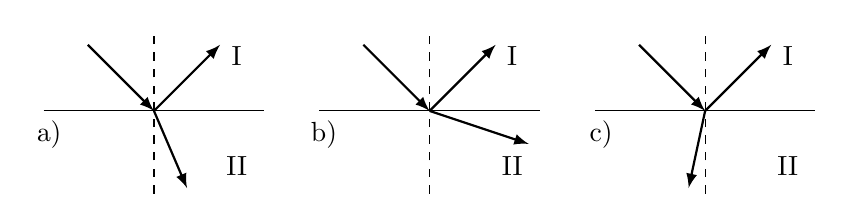
\begin{tikzpicture}[>=latex, scale=0.7]
    % --- a) grafik ---
    \begin{scope}[shift={(0,0)}]
        \draw (-2,0) -- (2,0); % Chegara
        \draw[dashed] (0,-1.5) -- (0,1.5); % Normal
        \draw[thick, ->] (-1.2,1.2) -- (0,0); % Tushayotgan
        \draw[thick, ->] (0,0) -- (1.2,1.2);  % Qaytayotgan
        \draw[thick, ->] (0,0) -- (0.6,-1.4); % Sinayotgan (yaqinlashgan)
        \node at (1.5,1) {I}; \node at (1.5,-1) {II};
        \node[below left] at (-1.5,0) {a)};
    \end{scope}

    % --- b) grafik ---
    \begin{scope}[shift={(5,0)}]
        \draw (-2,0) -- (2,0);
        \draw[dashed] (0,-1.5) -- (0,1.5);
        \draw[thick, ->] (-1.2,1.2) -- (0,0);
        \draw[thick, ->] (0,0) -- (1.2,1.2);
        \draw[thick, ->] (0,0) -- (1.8,-0.6); % Sinayotgan (uzoqlashgan)
        \node at (1.5,1) {I}; \node at (1.5,-1) {II};
        \node[below left] at (-1.5,0) {b)};
    \end{scope}

    % --- c) grafik ---
    \begin{scope}[shift={(10,0)}]
        \draw (-2,0) -- (2,0);
        \draw[dashed] (0,-1.5) -- (0,1.5);
        \draw[thick, ->] (-1.2,1.2) -- (0,0);
        \draw[thick, ->] (0,0) -- (1.2,1.2);
        \draw[thick, ->] (0,0) -- (-0.3,-1.4); % Sinayotgan (keskin yaqinlashgan)
        \node at (1.5,1) {I}; \node at (1.5,-1) {II};
        \node[below left] at (-1.5,0) {c)};
    \end{scope}
\end{tikzpicture}

\begin{enumerate}[label=\Alph*)]
\item a
\item a, b va c
\item c
\item a va b
\item b
\end{enumerate}

\item Sinish burchagi tushish burchagidan katta bo‘la oladimi?
\begin{enumerate}[label=\Alph*)]
\item hamma holda katta bo‘ladi.
\item nur optik zichligi kichikroq muhitdan optik zichligi kattaroq muhitga o‘tganda.
\item nur optik zichligi kattaroq muhitdan optik zichligi kichikroq muhitga o‘tganda.
\item nur vakuumdan muhitga o‘tganda.
\item bunday hol bo‘lmaydi.
\end{enumerate}

\item Rasmda ko‘rsatilgandek, yorug‘lik nuri ikki muhitning (1 va 2) ajralish chegarasidan o‘tadi. Quyidagilardan qaysi biri rasmdagi holatni to‘g‘ri ifodalaydi?

\begin{tikzpicture}[scale=0.8,>=latex]
    % Chegara va Normal
    \draw (-3,0) -- (3,0);
    \draw[dashed] (0,-1.5) -- (0,1.5);
    
    % Nurlar (O'ngdan tushib, chapga sinayotgan)
    \draw[thick, ->] (1.5, 1.5) -- (0,0);   % Tushayotgan nur
    \draw[thick, ->] (0,0) -- (-2, -0.8);   % Sinayotgan nur
    
    % Muhit nomlari
    \node at (-2, 1) {I};
    \node at (-2, -1) {II};
\end{tikzpicture}

\begin{enumerate}[label=\Alph*)]
\item yorug‘lik qutblangan.
\item 2-chi muhitda yorug‘lik tezligi 1-muhitdagidan katta.
\item 2-chi muhitda yorug‘lik tezligi 1-muhitdagidan kichik.
\item 1-muhitning absolyut sindirish ko‘rsatkichi birdan kichik.
\item TJY.
\end{enumerate}

\item Yorug‘lik nuri sindirish ko‘rsatkichi $n_1$ bo‘lgan muhitdan, sindirish ko‘rsatkichi $n_2$ bo‘lgan muhitga o‘tmoqda ($n_2>n_1$). Yorug‘lik muhitlar chegarasiga tiklik bilan $0^\circ$ burchak hosil qilib tushmoqda. Nurning sinish burchagi?
\begin{enumerate}[label=\Alph*)]
\item $\arcsin(n_1/n_2)$.
\item $\arcsin(n_2/n_1)$.
\item $0$.
\item $90^\circ$.
\item $\arcsin(1-n_2/n_1)$.
\end{enumerate}

\item Havoda sindirish ko‘rsatkichi $n=\sqrt{3}$ bo‘lgan muhitga nur tushganda, qaytgan nur bilan singan nur orasidagi burchak $90^\circ$ ga teng bo‘ldi. Nurning tushish burchagi qanday?
\begin{enumerate}[label=\Alph*)]
\item $0^\circ$
\item $30^\circ$
\item $45^\circ$
\item $60^\circ$
\item $90^\circ$
\end{enumerate}


\item Singan nur qaytgan nurga tik bo‘lishi uchun nur sindirish ko‘rsatkichi $n=1{,}732$ bo‘lgan shishaga havodan qanday burchak ostida tushishi kerak?
\begin{enumerate}[label=\Alph*)]
\item $30^\circ$.
\item $35^\circ16'$.
\item $45^\circ$.
\item $60^\circ$.
\item TJY.
\end{enumerate}

\item Singan nur qaytgan nurga tik bo‘lishi uchun nur yassi shishaga havodan qanday burchak ostida tushishi kerak? Shishaning sindirish ko‘rsatkichi $n$.
\begin{enumerate}[label=\Alph*)]
\item $\arccos n$.
\item $\arcsin n$.
\item $0$.
\item $\operatorname{arcctg} n$.
\item $\operatorname{arctg} n$.
\end{enumerate}

\item Yorug‘lik nuri suyuqlikdan vakuumga o‘tmoqda. Tushish burchagi $30^\circ$. Qaytgan va singan nurlar bir-biriga tik. Bu suyuqlikning sindirish ko‘rsatkichi qanday?
\begin{enumerate}[label=\Alph*)]
\item $1{,}3$.
\item $1{,}5$.
\item $1{,}73$.
\item $2$.
\item $2{,}5$.
\end{enumerate}

\item Sindirish ko‘rsatkichi $n$ ga teng muhitga yorug‘lik nuri havodan $\alpha$ burchak ostida tushmoqda. Qaytgan va singan nurlar orasidagi burchak $90^\circ$ ga teng bo‘lgan holat uchun $\alpha$ va $n$ orasidagi bog‘lanish qanday ko‘rinishda?
\begin{enumerate}[label=\Alph*)]
\item $tg\alpha=n$.
\item $\dfrac{\cos\alpha}{\sin\beta}=n$.
\item $\dfrac{\cos\alpha}{\cos\beta}=n$.
\item $\dfrac{\sin\alpha}{\cos\beta}=n$.
\item TJY.
\end{enumerate}

\item Yorug‘lik nuri sindirish ko‘rsatkichi $\sqrt{3}$ bo‘lgan shishadan havoga o‘tmoqda. Sinish burchagi tushish burchagidan 2 marta katta bo‘lishi uchun yorug‘lik havoga qanday burchak ostida tushishi kerak?
\begin{enumerate}[label=\Alph*)]
\item $25^\circ$.
\item $30^\circ$.
\item $45^\circ$.
\item $60^\circ$.
\item TJY.
\end{enumerate}

\item Yorug‘lik muhitdan havoga o‘tmoqda. Singan nur qaytgan nur bilan $90^\circ$ burchak tashkil etadi. Agar tushish burchagi sinusining qiymati $0{,}6$ ga teng bo‘lsa, sinish ko‘rsatkichi qanday?
\begin{enumerate}[label=\Alph*)]
\item $1$.
\item $1{,}25$.
\item $1{,}33$.
\item $1{,}5$.
\item $1{,}8$.
\end{enumerate}

\item Tushish burchagi $\alpha=0$ bo‘lganda, u sinish burchagi $\beta$ bilan qanday munosabatda bo‘ladi?
\begin{enumerate}[label=\Alph*)]
\item $\alpha=\beta$.
\item $\beta>\alpha$.
\item $\alpha>\beta$.
\item $\alpha=2\beta$.
\item $\beta=2\alpha$.
\end{enumerate}

\item Yorug‘lik nuri havodan suvga o‘tadi. Tushish burchagi $\alpha$ bo‘lsa, sinish burchagi $\beta$ quyidagi shartlardan qaysi birini qanoatlantiradi?
\begin{enumerate}[label=\Alph*)]
\item $\beta<\alpha$.
\item $\beta>\alpha$.
\item $\beta=\alpha$.
\item $\beta\gg\alpha$.
\item TJY.
\end{enumerate}

\item Yoqlari parallel bo‘lgan shaffof plastina orqali o‘tuvchi nurlarning qaysilarining yo‘li rasmda to‘g‘ri ko‘rsatilgan? Plastinani o‘rab turgan muhitning absolyut sindirish ko‘rsatkichi plastinkanikinidan katta.

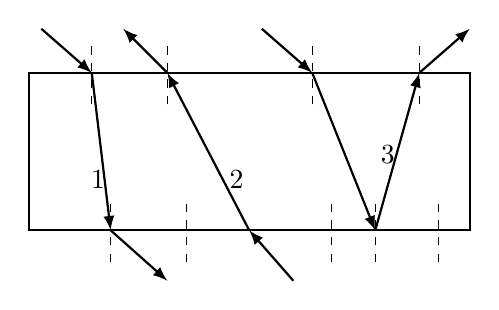
\begin{tikzpicture}[scale=0.8,>=latex]
    % Shaffof plastinka (to'rtburchak)
    \draw[thick] (0,0) rectangle (7,2.5);
    
    % Normallar (punktir chiziqlar)
    \foreach \x in {1, 2.2, 4.5, 6.2} {
        \draw[dashed] (\x, 2) -- (\x, 3); % Yuqori normallar
        \draw[dashed] (\x+0.3, -0.5) -- (\x+0.3, 0.5); % Pastki normallar
    }
    \draw[dashed] (5.5, -0.5) -- (5.5, 0.5); % 3-nur uchun pastki normal
    
    % 1-nur: Kirish va chiqish
    \draw[thick, ->] (0.2, 3.2) -- (1, 2.5);
    \draw[thick, ->] (1, 2.5) -- (1.3, 0);
    \draw[thick, ->] (1.3, 0) -- (2.2, -0.8);
    \node at (1.1, 0.8) {1};
    
    % 2-nur: Pastdan kirib yuqoridan chiqish
    \draw[thick, <-] (1.5, 3.2) -- (2.2, 2.5);
    \draw[thick, <-] (2.2, 2.5) -- (3.5, 0);
    \draw[thick, <-] (3.5, 0) -- (4.2, -0.8);
    \node at (3.3, 0.8) {2};
    
    % 3-nur: Qaytish (aks etish)
    \draw[thick, ->] (3.7, 3.2) -- (4.5, 2.5);
    \draw[thick, ->] (4.5, 2.5) -- (5.5, 0);
    \draw[thick, ->] (5.5, 0) -- (6.2, 2.5);
    \draw[thick, ->] (6.2, 2.5) -- (7, 3.2);
    \node at (5.7, 1.2) {3};
\end{tikzpicture}

\begin{enumerate}[label=\Alph*)]
\item 1.
\item 2.
\item 3.
\item 1 va 2.
\item 1 va 3.
\end{enumerate}

\item O‘quvchi prizmaning sindirish ko‘rsatkichini aniqlash uchun optik tajriba o‘tkazdi (rasm). Bu tajribaga asosan sindirish ko‘rsatkichi qaysi formula bo‘yicha aniqlanadi?

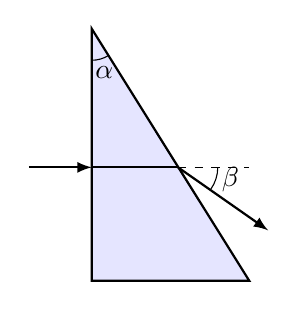
\begin{tikzpicture}[>=latex, scale=0.8]
    % Prizma (uchburchak)
    \draw[fill=blue!10, thick] (0,0) -- (0,4) -- (2.5,0) -- cycle;
    
    % Alfa burchagi (tepada)
    \draw (0, 3.5) arc (-90:-58:0.5);
    \node at (0.2, 3.3) {$\alpha$};
    
    % Tushayotgan nur (horizontal)
    \draw[thick, ->] (-1, 1.8) -- (0, 1.8);
    \draw[thick] (0, 1.8) -- (1.37, 1.8);
    
    % Normal chiziq (qiya sirtga perpendikulyar)
    \draw[rotate around={-58:(1.37,1.8)}] (0.7, 1.8) -- (2, 1.8);
    
    % Chiqayotgan (sinayotgan) nur
    \draw[thick, ->] (1.37, 1.8) -- (2.8, 0.8);
    
    % Beta burchagi uchun horizontal yordamchi chiziq
    \draw[dashed] (1.37, 1.8) -- (2.5, 1.8);
    \draw (2, 1.8) arc (0:-35:0.6);
    \node at (2.2, 1.6) {$\beta$};
\end{tikzpicture}

\begin{enumerate}[label=\Alph*)]
\item $\dfrac{\sin(\alpha+\beta)}{\sin\alpha}$.
\item $\dfrac{\sin(\alpha-\beta)}{\sin\alpha}$.
\item $\dfrac{\sin(\alpha+\beta)}{2\sin\alpha}$.
\item $\dfrac{\sin(\alpha+\beta)}{\cos\alpha}$.
\item $\dfrac{\sin(\alpha+\beta)}{2\cos\alpha}$.
\end{enumerate}

\item Agar yorug‘lik nuri yassi parallel shisha ($n=1{,}7$) plastinkaga $53^\circ$ burchak ostida tushib, undan o‘tishda $2$ cm masofa siljigan bo‘lib, $\sin53^\circ=0{,}8$, (cm).
\begin{enumerate}[label=\Alph*)]
\item $1{,}8$.
\item $2{,}6$.
\item $3{,}4$.
\item $1{,}6$.
\item $4{,}2$.
\end{enumerate}

\item Muntazam uchburchakli prizmaning yon tomoniga $45^\circ$ burchak ostida nur tushmoqda. Nur prizmadan chiqishda dastlabki yo‘nalishga nisbatan qanday burchakka og‘adi? $n=\sqrt{2}$, $\sin45^\circ=\sqrt{2}/2$.
\begin{enumerate}[label=\Alph*)]
\item $15^\circ$.
\item $30^\circ$.
\item $45^\circ$.
\item $60^\circ$.
\item $90^\circ$.
\end{enumerate}

\end{enumerate}

\begin{center}
\renewcommand{\arraystretch}{1.2}
\begin{tabular}{|c|c|c|c|c|c|c|c|c|c|}
\hline
1b & 2d & 3c & 4c & 5c & 6b & 7d & 8d & 9b & 10d \\
\hline
11d & 12d & 13c & 14b & 15d & 16b & 17a & 18d & 19b & 20e \\
\hline
21c & 22b & 23a & 24d & 25d & 26e & 27c & 28a & 29b & 30c \\
\hline
31a & 32a & 33b & 34a & 35e & 36b & & & & \\
\hline
\end{tabular}
\end{center}






\section{ Yorug‘likning to‘lqin tabiati}

\begin{enumerate}

\item Kerosinning dielektrik singdiruvchanligi $2$, magnit kirituvchanligi $1$ bo‘lsa, absolyut sindirish ko‘rsatkichi qanday?
\begin{enumerate}[label=\Alph*)]
\item $1$.
\item $1,5$.
\item $2$.
\item $2\sqrt{2}$.
\item $\sqrt{2}$.
\end{enumerate}

\item Sindirish ko‘rsatkichi $n$ bo‘lgan shaffof jismga vakuumdan yorug‘lik tushayapti. Agar yorug‘likning vakuumdagi tezligi $c$ bo‘lsa, uning jism ichidagi tezligi qanday bo‘ladi?
\begin{enumerate}[label=\Alph*)]
\item $c/n$.
\item $nc$.
\item $c$.
\item $n/c$.
\item $\sqrt{nc}$.
\end{enumerate}

\item Absolyut sindirish ko‘rsatkichi $1,5$ bo‘lgan muhitdagi yorug‘lik tezligi qanday (m/s)?
\begin{enumerate}[label=\Alph*)]
\item $1,5\cdot10^7$.
\item $2\cdot10^8$.
\item $2\cdot10^7$.
\item $1,5\cdot10^8$.
\item $1\cdot10^7$.
\end{enumerate}

\item Absolyut sindirish ko‘rsatkichi $2,5$ bo‘lgan muhitda yorug‘lik qanday tezlik bilan tarqaladi?
\begin{enumerate}[label=\Alph*)]
\item $0,8c$.
\item $0,14c$.
\item $0,7c$.
\item $c$.
\item $0,4c$.
\end{enumerate}

\item Sindirish ko‘rsatkichi $n_1=1,4$ va sinish ko‘rsatkichi $n_2=1,75$ bo‘lgan muhitlarda tarqalayotgan nurlarning tezliklari nisbati qanday?
\begin{enumerate}[label=\Alph*)]
\item $1,1$.
\item $1,15$.
\item $1,25$.
\item $1,2$.
\item $1,3$.
\end{enumerate}

\item Nurning shaffof muhitdagi tezligi $0,25c$ ga teng. Muhitning absolyut sindirish ko‘rsatkichini aniqlang. $c$ — yorug‘likning vakuumdagi tezligi.
\begin{enumerate}[label=\Alph*)]
\item $1,33$.
\item $1,5$.
\item $4$.
\item $2$.
\item $2,3$.
\end{enumerate}

\item Yorug‘lik tezligi $0,625c$ ga teng bo‘lgan muhitning absolyut sindirish ko‘rsatkichini toping, $c$ — yorug‘likning vakuumdagi tezligi.
\begin{enumerate}[label=\Alph*)]
\item $2$.
\item $1,8$.
\item $1,7$.
\item $1,6$.
\item $1,5$.
\end{enumerate}

\item Yorug‘lik to‘lqinining havodagi uzunligi $0,6~\mu$m. Uning suvdagi to‘lqin uzunligi necha $\mu$m bo‘ladi? Suvning sindirish ko‘rsatkichi $n=4/3$.
\begin{enumerate}[label=\Alph*)]
\item $0,8$.
\item $0,64$.
\item $0,6$.
\item $0,5$.
\item $0,45$.
\end{enumerate}

\item Havodagi uzunligi $450$ nm bo‘lgan yorug‘lik to‘lqinining shishadagi uzunligi qanday (nm)? Shishaning sindirish ko‘rsatkichi $1,5$ ga teng.
\begin{enumerate}[label=\Alph*)]
\item $150$.
\item $675$.
\item $300$.
\item $250$.
\item $200$.
\end{enumerate}

\item To‘lqin uzunligi $5\cdot10^{-7}$ m bo‘lgan yorug‘likning tebranish chastotasi necha Gersga teng? $c=3\cdot10^8$ m/s.
\begin{enumerate}[label=\Alph*)]
\item $6\cdot10^{15}$.
\item $0,6\cdot10^{15}$.
\item $6\cdot10^{12}$.
\item $6\cdot10^{13}$.
\item $0,6\cdot10^{14}$.
\end{enumerate}

\item Vakuumdagi to‘lqin uzunligi $0,75~\mu$m bo‘lgan yorug‘likning chastotasini toping (Hz).
\begin{enumerate}[label=\Alph*)]
\item $5\cdot10^{14}$.
\item $4\cdot10^{15}$.
\item $7,5\cdot10^{14}$.
\item $5\cdot10^{15}$.
\item $4\cdot10^{14}$.
\end{enumerate}

\item Vakuumdagi yorug‘likning to‘lqin uzunligi $\lambda=6\cdot10^{-7}$ m. Uning tebranishlar chastotasi necha Gers?
\begin{enumerate}[label=\Alph*)]
\item $6\cdot10^{15}$.
\item $5\cdot10^{15}$.
\item $1,8\cdot10^{15}$.
\item $5\cdot10^{14}$.
\item $6\cdot10^7$.
\end{enumerate}

\item Agar muhitda tarqalayotgan yorug‘likning chastotasi $3\cdot10^{14}$ Hz, to‘lqin uzunligi $500$ nm bo‘lsa, muhitning sindirish ko‘rsatkichi qanday?
\begin{enumerate}[label=\Alph*)]
\item $2$.
\item $1,7$.
\item $1,6$.
\item $1,5$.
\item $1,33$.
\end{enumerate}

\item Chastotasi $3\cdot10^{14}$ Hz bo‘lgan yorug‘likning sindirish ko‘rsatkichi $2$ ga teng bo‘lgan muhitdagi to‘lqin uzunligini aniqlang (nm).
\begin{enumerate}[label=\Alph*)]
\item $200$.
\item $400$.
\item $450$.
\item $500$.
\item $600$.
\end{enumerate}

\item Agar olmosda chastotasi $2,73\cdot10^{14}$ Hz bo‘lgan yorug‘lik to‘lqinining uzunligi $450$ nm bo‘lsa, yorug‘likning olmosdagi tezligi qanday (m/s)?
\begin{enumerate}[label=\Alph*)]
\item $1,23\cdot10^8$.
\item $2,23\cdot10^8$.
\item $2,5\cdot10^8$.
\item $1,5\cdot10^8$.
\item $2,83\cdot10^8$.
\end{enumerate}

\item Monoxromatik yorug‘lik bir muhitdan ikkinchi muhitga o‘tganda, to‘lqin uzunligi $2$ marta kamaygan bo‘lsa, uning tarqalish tezligi qanday o‘zgargan?
\begin{enumerate}[label=\Alph*)]
\item $2$ marta kamaygan.
\item $\sqrt{2}$ marta kamaygan.
\item $\sqrt{2}$ marta oshgan.
\item $2$ marta oshgan.
\item o‘zgarmagan.
\end{enumerate}

\item Shaffof muhitdagi yorug‘lik chastotasi $4\cdot10^{14}$ Hz, to‘lqin uzunligi $500$ nm bo‘lsa, muhitning sindirish ko‘rsatkichi qanday?
\begin{enumerate}[label=\Alph*)]
\item $1,33$.
\item $1,5$.
\item $1,7$.
\item $2$.
\item $2,25$.
\end{enumerate}

\item Muhitda yorug‘likning to‘lqin uzunligi $400$ nm, chastotasi $5\cdot10^{14}$ Hz bo‘lsa, shu muhitning sindirish ko‘rsatkichi nimaga teng?
\begin{enumerate}[label=\Alph*)]
\item $1,7$.
\item $1,6$.
\item $7,3$.
\item $1,4$.
\item $1,5$.
\end{enumerate}

\item Yashil yorug‘lik muz sirtiga $45^\circ$ burchak ostida tushib, $33^\circ$ burchak ostida sindi. Yorug‘lik muzda necha m/s tezlik bilan tarqaladi? $\sin45^\circ=0,7$, $\sin33^\circ=0,54$ deb hisoblang.
\begin{enumerate}[label=\Alph*)]
\item $3\cdot10^8$.
\item $2,3\cdot10^8$.
\item $1,3\cdot10^8$.
\item $2\cdot10^8$.
\item $1,5\cdot10^8$.
\end{enumerate}

\item Agar yorug‘lik qavariq suv tomchisi orqali bir vaqtda $45$ cm masofaga o‘tsa, biror suyuqlikda esa shunday vaqtda $30$ cm masofaga o‘tsa, bu suyuqlikning sindirish ko‘rsatkichi nimaga teng?
\begin{enumerate}[label=\Alph*)]
\item $1,2$.
\item $1,3$.
\item $1,4$.
\item $1,5$.
\item $1,7$.
\end{enumerate}

\item Sindirish ko‘rsatkichi $n_1=1,2$, skipidarniki $n_2=1,5$. Shu moddalardan yorug‘lik bir xil vaqtda o‘tadigan yo‘llar nisbati nimaga teng?
\begin{enumerate}[label=\Alph*)]
\item $1,22$.
\item $1,21$.
\item $1,2$.
\item $1,25$.
\item TJY.
\end{enumerate}

\item Nurning ikki muhit chegarasiga tushish burchagi $30^\circ$ bo‘lganda, sinish burchagi $45^\circ$ bo‘lsa, yorug‘lik birinchi muhitdan ikkinchi muhitga o‘tganda, tezlik qanday o‘zgaradi?
\begin{enumerate}[label=\Alph*)]
\item $1,5$ marta oshadi.
\item $\sqrt{2}$ marta kamayadi.
\item $\sqrt{2}$ marta oshadi.
\item $2$ marta kamayadi.
\item $2$ marta oshadi.
\end{enumerate}

\item Elektromagnit tebranishlar chastotasi $10^{15}$ Hz bo‘lsa, sindirish ko‘rsatkichi $1,5$ ga teng bo‘lgan muhitda yorug‘lik to‘lqini uzunligi necha metr? Yorug‘likning bo‘shliqdagi tezligi $3\cdot10^8$ m/s ga teng.
\begin{enumerate}[label=\Alph*)]
\item $2\cdot10^{-7}$.
\item $3\cdot10^{-7}$.
\item $0,5\cdot10^{-7}$.
\item $0,3\cdot10^{-7}$.
\item yorug‘lik to‘lqinining uzunligini berilgan kattaliklar asosida aniqlab bo‘lmaydi.
\end{enumerate}

\item Havodagi uzunligi $720$ nm bo‘lgan yorug‘lik to‘lqinining olmosdagi uzunligi qanday (nm)? Yorug‘likning olmosdagi tezligi $1,25\cdot10^8$ m/s.
\begin{enumerate}[label=\Alph*)]
\item $250$.
\item $300$.
\item $360$.
\item $576$.
\item $900$.
\end{enumerate}

\item Yorug‘lik vakuumda sindirish ko‘rsatkichi $n$ bo‘lgan muhitga o‘tayapti. Quyidagi fikrlardan qaysisi to‘g‘ri?
\begin{enumerate}[label=\Alph*)]
\item chastotasi va tezligi o‘zgarmaydi.
\item to‘lqin uzunligi va tezligi $n$ marta kamayadi.
\item chastotasi va to‘lqin uzunligi $n$ marta kamayadi.
\item to‘lqin uzunligi $n$ marta ortadi, chastotasi $n$ marta kamayadi.
\item chastotasi $n$ marta ortadi, to‘lqin uzunligi $n$ marta kamayadi.
\end{enumerate}

\item Yorug‘lik vakuumdan sindirish ko‘rsatkichi $n=2$ bo‘lgan muhitga o‘tganda to‘lqin uzunligi qanday o‘zgaradi?
\begin{enumerate}[label=\Alph*)]
\item $2$ marta ortadi.
\item $2$ marta kamayadi.
\item o‘zgarmaydi.
\item o‘zgarish tushish burchagiga bog‘liq bo‘ladi.
\item TJY.
\end{enumerate}

\item Havodan optik muhitga o‘tgan nurning to‘lqin uzunligi $30\%$ kamaydi. Nurning bu muhitdagi tezligi nimaga teng?
\begin{enumerate}[label=\Alph*)]
\item $0,3c$.
\item $0,7c$.
\item $0,49c$.
\item $0,8c$.
\item $0,6c$.
\end{enumerate}

\item Absolyut sindirish ko‘rsatkichi $2$ bo‘lgan muhitdan absolyut sindirish ko‘rsatkichi $1,5$ bo‘lgan muhitga o‘tishda yorug‘likning to‘lqin uzunligi qanday o‘zgaradi?
\begin{enumerate}[label=\Alph*)]
\item o‘zgarmaydi.
\item $3$ marta kamayadi.
\item $3$ marta ortadi.
\item $4/3$ marta kamayadi.
\item $4/3$ marta ortadi.
\end{enumerate}

\item Monoxromatik yorug‘lik uch muhitdan ketma-ket o‘tganda shu muhitlardagi to‘lqin uzunligi $\lambda_1=550$ nm; $\lambda_2=550{,}1$ nm va $\lambda_3=549{,}5$ nm bo‘ldi. Bu muhitlarning sindirish ko‘rsatkichlari uchun quyidagi munosabatlardan qaysi biri o‘rinli?
\begin{enumerate}[label=\Alph*)]
\item $n_1>n_2>n_3$.
\item $n_3>n_1>n_2$.
\item $n_1<n_2<n_3$.
\item $n_1=n_2=n_3$.
\item $n_2>n_3>n_1$.
\end{enumerate}

\item Yorug‘lik to‘lqini vakuumdan muhitga o‘tganda, to‘lqin uzunligi $1,5$ marta kamaydi. Yorug‘likning shu muhitdagi tezligini (m/s) aniqlang.
\begin{enumerate}[label=\Alph*)]
\item $1,5\cdot10^8$.
\item $1\cdot10^8$.
\item $0,5\cdot10^8$.
\item $2\cdot10^8$.
\item $2,5\cdot10^8$.
\end{enumerate}

\item Yorug‘lik birinchi muhitdan ikkinchi muhitga $\alpha_1$ burchak ostida tushadi. Sinish burchagi $\alpha_2$. Birinchi muhitda yorug‘likning to‘lqin uzunligi $\lambda_1$ bo‘lsa, ikkinchi muhitda to‘lqin uzunligi $\lambda_2$ qanday bo‘ladi?
\begin{enumerate}[label=\Alph*)]
\item $\lambda_2=\lambda_1\sin\alpha_2/\alpha_1$.
\item $\lambda_2=\lambda_1 tg\alpha_1/\alpha_2$.
\item $\lambda_2=\lambda_1\sin\alpha_2/\sin\alpha_1$.
\item $\lambda_2=\lambda_1\sin\alpha_1/\sin\alpha_2$.
\item $\lambda_2=\lambda_1 tg\alpha_2/ tg\alpha_1$.
\end{enumerate}


\item Agar to‘lqin uzunligi $4\cdot10^{-7}$ m bo‘lgan yorug‘lik nuri bir muhitdan ikkinchi muhitga tushish burchagi $30^\circ$, sinish burchagi $45^\circ$ bo‘lsa, ikkinchi muhitdagi to‘lqin uzunligi necha nm?
\begin{enumerate}[label=\Alph*)]
\item $283$.
\item $320$.
\item $400$.
\item $566$.
\item $800$.
\end{enumerate}

\item Birinchi muhitdagi to‘lqin uzunligi $560$ nm bo‘lgan yorug‘lik nurining ikkinchi muhitga tushish burchagi $45^\circ$, sinish burchagi $30^\circ$ bo‘lsa, ikkinchi muhitdagi to‘lqin uzunligi necha nanometr? $\sqrt{2}\approx1{,}4$.
\begin{enumerate}[label=\Alph*)]
\item $840$.
\item $784$.
\item $560$.
\item $400$.
\item $373$.
\end{enumerate}

\item Chastotasi $5\cdot10^{14}$ Hz bo‘lgan yorug‘likning sindirish ko‘rsatkichi $1,5$ bo‘lgan muhitdagi to‘lqin uzunligini aniqlang (nm).
\begin{enumerate}[label=\Alph*)]
\item $300$.
\item $400$.
\item $500$.
\item $600$.
\item $750$.
\end{enumerate}

\item Sindirish ko‘rsatkichi $1,5$ bo‘lgan shaffof muhitda tarqalayotgan, to‘lqin uzunligi $500$ nm bo‘lgan yorug‘likning chastotasini aniqlang (Hz)?
\begin{enumerate}[label=\Alph*)]
\item $5\cdot10^{15}$.
\item $4\cdot10^{14}$.
\item $1,5\cdot10^{15}$.
\item $3\cdot10^{14}$.
\item $4\cdot10^{15}$.
\end{enumerate}

\item Agar $600$ nm to‘lqin uzunlikdagi yorug‘lik vakuumdan biror muhitga o‘tganda, tezligi $40\%$ ga kamaygan bo‘lsa, yorug‘lik shu muhitdagi to‘lqin uzunligi qanday (nm)?
\begin{enumerate}[label=\Alph*)]
\item $240$.
\item $360$.
\item $750$.
\item $1000$.
\item $1500$.
\end{enumerate}

\item Yorug‘lik to‘lqini bir muhitdan boshqasiga o‘tmoqda. Unga tegishli qaysi kattaliklar o‘zgaradi?
\begin{enumerate}[label=\Alph*)]
\item to‘lqin uzunligi;
\item chastota;
\item tarqalish tezligi;
\item amplituda.
\end{enumerate}

\begin{enumerate}[label=\Alph*)]
\item faqat 2.
\item 2, 4.
\item 2, 3, 4.
\item 1, 4.
\item 4.
\end{enumerate}

\item Elektromagnit to‘lqinlar bir muhitdan ikkinchi muhitga o‘tganda, quyidagi hodisalarning qaysi biri yuz beradi?
\begin{enumerate}[label=\Alph*)]
\item faqat chastota o‘zgaradi.
\item hech qanday o‘zgarish bo‘lmaydi.
\item to‘lqin uzunligi va chastota o‘zgaradi.
\item chastota va tezlik o‘zgaradi.
\item to‘lqin uzunligi va tezlik o‘zgaradi.
\end{enumerate}

\item Yorug‘lik bir muhitdan ikkinchi muhitga o‘tganda, uning chastotasi, tezligi va to‘lqin uzunligidan qaysilari o‘zgarmaydi?
\begin{enumerate}[label=\Alph*)]
\item to‘lqin uzunligi.
\item tezligi va to‘lqin uzunligi.
\item tezligi.
\item chastotasi.
\item chastotasi va tezligi.
\end{enumerate}

\item Monoxromatik yorug‘lik vakuumdan sindirish ko‘rsatkichi $n=2$ bo‘lgan muhitga o‘tganda, uning chastotasi qanday o‘zgaradi?
\begin{enumerate}[label=\Alph*)]
\item $4$ marta ortadi.
\item $2$ marta kamayadi.
\item $2$ marta ortadi.
\item $4$ marta kamayadi.
\item o‘zgarmaydi.
\end{enumerate}

\item Chastotasi $3\cdot10^{15}$ Hz bo‘lgan elektromagnit to‘lqin vakuumdan sindirish ko‘rsatkichi $1,5$ ga teng bo‘lgan muhitga o‘tganda, uning chastotasi necha bo‘ladi?
\begin{enumerate}[label=\Alph*)]
\item $4,5\cdot10^{15}$.
\item $5\cdot10^{14}$.
\item $2\cdot10^{15}$.
\item $1,5\cdot10^{15}$.
\item $3\cdot10^{15}$.
\end{enumerate}

\item Absolyut sindirish ko‘rsatkichi $2$ bo‘lgan muhitdan absolyut sindirish ko‘rsatkichi $1,33$ bo‘lgan muhitga o‘tganda yorug‘lik to‘lqinining chastotasi qanday o‘zgaradi?
\begin{enumerate}[label=\Alph*)]
\item o‘zgarmaydi.
\item $3$ marta kamayadi.
\item $1,5$ marta kamayadi.
\item $3$ marta ortadi.
\item $1,5$ marta ortadi.
\end{enumerate}

\item Agar elektromagnit tebranishlar chastotasi vakuumda $1$ MHz bo‘lsa, sindirish ko‘rsatkichi $2$ ga teng bo‘lgan bir jinsli muhitda chasto ta necha MHz bo‘ladi?
\begin{enumerate}[label=\Alph*)]
\item $0,2$.
\item $0,5$.
\item $0,8$.
\item $1$.
\item $2$.
\end{enumerate}

\item $7{,}5\cdot10^{14}$ Hz chastotali (vakuumda) yorug‘lik sindirish ko‘rsatkichlari $n_1=1$, $n_2=1,5$ va $n_3=1,6$ bo‘lgan muhitlardan ketma-ket o‘tmoqda. Bu muhitlardagi yorug‘lik chastotalari uchun qaysi munosabat o‘rinli?
\begin{enumerate}[label=\Alph*)]
\item $\nu_1>\nu_2<\nu_3$.
\item $\nu_3>\nu_1>\nu_2$.
\item $\nu_1<\nu_2<\nu_3$.
\item $\nu_2>\nu_1>\nu_3$.
\item $\nu_1=\nu_2=\nu_3$.
\end{enumerate}

\item $480$ nm to‘lqin uzunlikdagi yorug‘lik vakuumdan biror muhitga o‘tganda, to‘lqin uzunligi $192$ nm ga qisqardi. Yorug‘likning shu muhitdagi tezligini toping (m/s).
\begin{enumerate}[label=\Alph*)]
\item $1\cdot10^8$.
\item $1,2\cdot10^8$.
\item $1,8\cdot10^8$.
\item $2\cdot10^8$.
\item $1,5\cdot10^8$.
\end{enumerate}

\item Nurlar suvdan vakuumga o‘tganda ularning to‘lqin uzunligi $0,165~\mu$m ga ortdi. Nurlarning vakuumdagi to‘lqin uzunligini aniqlang ($\mu$m). $n=1,33$.
\begin{enumerate}[label=\Alph*)]
\item $0,365$.
\item $0,41$.
\item $0,56$.
\item $0,605$.
\item $0,665$.
\end{enumerate}

\item Yassi yorug‘lik ikki muhit chegarasiga $\alpha$ burchak ostida tushib, $\beta$ burchak ostida ikkinchi muhitga o‘tmoqda. Yorug‘likning shu muhitlardagi tarqalish tezliklari qanday munosabatda bo‘ladi? $\alpha>\beta$.
\begin{enumerate}[label=\Alph*)]
\item tezliklar munosabati ga bog‘liq o‘zgaradi.
\item $v_1<v_2$.
\item $v_1>v_2$.
\item $v_1=v_2$.
\item TJY.
\end{enumerate}

\item Yorug‘lik 1-muhitdan 2-muhitga $45^\circ$ burchak ostida tushib, 2-muhitda $30^\circ$ burchak ostida sinib o‘tadi. 1-muhitning absolyut sindirish ko‘rsatkichi $\sqrt{2}$ ga teng bo‘lsa, yorug‘likning 2-muhitdagi tezligi necha km/s ga teng bo‘ladi? $\sin45^\circ=\sqrt{2}/2$, $\sin30^\circ=1/2$.
\begin{enumerate}[label=\Alph*)]
\item $\sqrt{2}\cdot150000$.
\item $300000/\sqrt{2}$.
\item $200000$.
\item $300000$.
\item $150000$.
\end{enumerate}

\item Qanday muhitda yorug‘lik nurlari egri chiziq bo‘lib yurishi mumkin?
\begin{enumerate}[label=\Alph*)]
\item bir jinsli muhitda.
\item suyuq muhitda.
\item monokristalda.
\item amorf moddada.
\item sindirish ko‘rsatkichi nuqtadan nuqtaga o‘zgaruvchi muhitda.
\end{enumerate}

\item Yorug‘likning qandaydir shaffof muhitdagi tezligi $1,5\cdot10^8$ m/s bo‘lsa, shu muhitning dielektrik singdiruvchanligi qanday?
\begin{enumerate}[label=\Alph*)]
\item $1,5$.
\item $2$.
\item $3$.
\item $4$.
\item $8$.
\end{enumerate}

\end{enumerate}

\begin{center}
\renewcommand{\arraystretch}{1.2}
\begin{tabular}{|c|c|c|c|c|c|c|c|c|c|}
\hline
1e & 2a & 3b & 4e & 5c & 6c & 7d & 8e & 9c & 10b \\
\hline
11e & 12d & 13a & 14d & 15a & 16a & 17b & 18e & 19b & 20d \\
\hline
21d & 22c & 23a & 24b & 25b & 26b & 27b & 28e & 29b & 30d \\
\hline
31c & 32d & 33d & 34b & 35b & 36b & 37a & 38e & 39d & 40e \\
\hline
41e & 42a & 43d & 44e & 45c & 46a & 47c & 48e & 49e & 50d \\
\hline
\end{tabular}
\end{center}












